\date{}
\title{barriers (finish) / deadlock}
\date{}
\begin{document}
\begin{frame}
    \titlepage
\end{frame}


\makeatletter
\newenvironment<>{btHighlight}[1][]
{\begin{onlyenv}#2\begingroup\tikzset{bt@Highlight@par/.style={#1}}\begin{lrbox}{\@tempboxa}}
{\end{lrbox}\bt@HL@box[bt@Highlight@par]{\@tempboxa}\endgroup\end{onlyenv}}

\newcommand<>\btHL[1][]{%
  \only#2{\begin{btHighlight}[#1]\bgroup\aftergroup\bt@HL@endenv}%
}
\def\bt@HL@endenv{%
  \end{btHighlight}%   
  \egroup %
}
\tikzset{
    btHLbox/.style={
        fill=red!30,outer sep=0pt,inner xsep=1pt, inner ysep=0pt, rounded corners=3pt
    },
}
\newcommand{\bt@HL@box}[2][]{%
  \tikz[#1]{%
    \pgfpathrectangle{\pgfpoint{1pt}{0pt}}{\pgfpoint{\wd #2}{\ht #2}}%
    \pgfusepath{use as bounding box}%
    \node[text width={},draw=none,anchor=base west, btHLbox, minimum height=\ht\strutbox+1pt,#1]{\raisebox{1pt}{\strut}\strut\usebox{#2}};
  }%
}

\lst@CCPutMacro
    \lst@ProcessOther {"2A}{%
      \lst@ttfamily 
         {\raisebox{2pt}{*}}% used with ttfamily
         {\raisebox{2pt}{*}}}% used with other fonts
    \@empty\z@\@empty

\lstdefinelanguage
   [x8664gas]{Assembler}     % add a "x64" dialect of Assembler
   [x86masm]{Assembler} % based on the "x86masm" dialect
   % with these extra keywords:
   {morekeywords={CDQE,CQO,CMPSQ,CMPXCHG16B,JRCXZ,LODSQ,MOVSXD,%
                  POPFQ,PUSHFQ,SCASQ,STOSQ,IRETQ,RDTSCP,SWAPGS,.TEXT,.STRING,.ASCIZ,%
                  BEQ,LW,SW,LB,SB,ADDIU,J,BEQZ,BNEZ,BNE,%
                  MOVUPD,MULPD,MOVSD,MULSD,%
                  SHLADD,MOV,CMP.LT,TBIT.NZ,BR.RET.SPTK.MANY,%
                  ADDQ,POPQ,PUSHQ,RRMOVQ,MRMOVQ,RMMOVQ,IRMOVQ,%
                  <-,LL,SC,ADDI,ADDL,VMOVDQA,ADDQ,CMPL,JB,JBE,MOVL,CLTQ,
                  MOVW,PUSHW,MOV,ADD,SUB,INT,PUSH,MOV,ADD,REP,MOVSB,%
                  TESTQ,CMPQ,MOVL,MOVQ,ADDQ,JMPQ,XORQ,%
                  LEAQ,LEAL,LEA,RETQ,RET,POPL,POPW,PUSHL,PUSHW,%
                  LEAW,%
                  SUBQ,SYSCALL,.ASCII,CALLQ,MOVSLQ,JMP,ANDQ,SHRQ,MOVB,INCQ,TESTL,XORL,%
                  SHRL,LEAL,SARL,SUBL,IMULL,IMULQ,MOVDQU,PADDD,XORL,%
                  MOVZBL,MOVZB,SHRB,SRAL,SHRL,ANDL,%
                  CMOVNS,SRAL,SRAQ,MOVZBW,MOVZBQ,%
                  PADDW,PADDQ,MODUPS,MOVAPD,%
                  MOVL,RET,.GLOBL,%
                  },
    deletekeywords={eax,ebx,sp,si,cx,di,ds,cs,es,fs,dx,ax,bx,al,esi,ebp,ecx,rip,eip,edx,edi,rdi,esp},
    morecomment=[l]{\#},
    morecomment=[l]{\/\/},
    morecomment=[s]{/*}{*/},
    sensitive=false,
    keepspaces=true} % et

\lstalias[]{myasm}[x8664gas]{Assembler}

\lstdefinelanguage{JavaScript}{
  keywords={typeof, new, true, false, catch, function, return, null, catch, switch, var, if, in, while, do, else, case, break},
  ndkeywords={class, export, boolean, throw, implements, import, this},
  sensitive=false,
  comment=[l]{//},
  morecomment=[s]{/*}{*/},
  morestring=[b]',
  morestring=[b]"
}

\newcommand{\keywordstyle}{\sourcecodeprolight\bfseries\color{blue!30!black}}
\newcommand{\stringstyle}{\color{blue!20!black}\ttfamily}

\lstset{
    language=C,
    basicstyle=\sourcecodepro\EmptyMapping,
    escapechar=`,
    keywordstyle=\keywordstyle\EmptyMapping,
    identifierstyle=\sourcecodepro\EmptyMapping,
    numberstyle=\small\color{black!70},
    commentstyle=\color{red!60!black}\ttfamily\itshape,
    stringstyle=\color{blue!20!black}\ttfamily,
    ndkeywordstyle=\bfseries\color{blue!30!black},
    upquote=true,
}



\lstdefinestyle{medium}{
    basicstyle=\sourcecodepro\EmptyMapping\fontsize{12}{13}\selectfont,
    keywordstyle=\sourcecodepro\EmptyMapping\fontsize{12}{13}\selectfont\keywordstyle,
}

\lstdefinestyle{small}{
    basicstyle=\sourcecodepro\EmptyMapping\small,
    keywordstyle=\sourcecodepro\EmptyMapping\small\keywordstyle,
}

\lstdefinestyle{smaller}{
    basicstyle=\sourcecodepro\EmptyMapping\fontsize{11}{12}\selectfont,
    keywordstyle=\sourcecodepro\EmptyMapping\fontsize{11}{12}\selectfont\keywordstyle,
}


\lstdefinestyle{script}{
    basicstyle=\sourcecodepro\EmptyMapping\scriptsize,
    keywordstyle=\sourcecodepro\EmptyMapping\scriptsize\bfseries,
}




\begin{frame}{last time}
    \begin{itemize}
    \item race conditions
        \begin{itemize}
        \item inconsistent results due to timing variation
        \item example: ``lose'' update due to reading value while update being computed
        \end{itemize}
    \item compilers, processors and memory access reordering
        \begin{itemize}
        \item order you write in C code [or even assembly] might not be order of accesses
        \item need special operations that gaurentee consistent order
        \end{itemize}
    \item locks for taking turns
        \begin{itemize}
        \item one thread can ``hold'' lock at a time
        \item lock operation waits for lock to be available (unlock'd)
        \item requires threads agree to get lock before using shared thing
        \end{itemize}
    \item barriers --- advance threads in lock-step
    \end{itemize}
\end{frame}

\section{barriers}
\subsection{exercise}
\begin{frame}[fragile]{exercise}
\lstset{language=C,style=smaller}
\begin{lstlisting}
pthread_barrier_t barrier;
int x = 0, y = 0;
void thread_one() {
    y = 10;
    pthread_barrier_wait(&barrier);
    y = x + y;
    pthread_barrier_wait(&barrier);
    pthread_barrier_wait(&barrier);
    printf("%d %d\n", x, y);
}

void thread_two() {
    x = 20;
    pthread_barrier_wait(&barrier);
    pthread_barrier_wait(&barrier);
    x = x + y;
    pthread_barrier_wait(&barrier);
}
\end{lstlisting}
\begin{itemize}
\item if both thread\_one, thread\_two run at once
\item output? 
\end{itemize}
\end{frame}


\usetikzlibrary{arrows.meta,shapes.geometric}
\tikzset{
    >=Latex,
    resource/.style={draw,rectangle,very thick,align=center},
    resource m/.style={draw,rectangle,very thick,align=center,row sep=2mm},
    resource circle/.style={circle,fill=black,inner sep=0mm,minimum width=2.5mm},
    thread/.style={draw,ellipse,very thick,align=center},
    dependency/.style={draw,ultra thick,->},
    dependency future/.style={dependency,dotted},
    dependency reason/.style={align=center},
}

\usetikzlibrary{arrows.meta,shapes.geometric}
\tikzset{
    >=Latex,
    resource/.style={draw,rectangle,very thick,align=center},
    resource m/.style={draw,rectangle,very thick,align=center,row sep=2mm},
    resource circle/.style={circle,fill=black,inner sep=0mm,minimum width=2.5mm},
    thread/.style={draw,ellipse,very thick,align=center},
    dependency/.style={draw,ultra thick,->},
    dependency future/.style={dependency,dotted},
    dependency reason/.style={align=center},
}


\section{deadlock examples}

\subsection{a one-way bridge}
\begin{frame}{the one-way bridge}
\begin{tikzpicture}
\tikzset{
    bridge line/.style={ultra thick},
    road divide/.style={very thick,loosely dashed},
    old car black/.pic={
        \node at (0,-0.25) {
\includegraphics[width=1.25cm,angle=-90,origin=c]{../deadlock/Car_icon_top.pdf}};
    },
    old car black opposite/.pic={
        \node at (0,-0.25) {
\includegraphics[width=1.25cm,angle=90,origin=c]{../deadlock/Car_icon_top.pdf}};
    },
    old car black opposite rot/.pic={
        \node at (0,-0.25) {
\includegraphics[width=1.25cm,angle=85,origin=c]{../deadlock/Car_icon_top.pdf}};
    },
    old car red/.pic={
        \node at (0,-0.25) {
\includegraphics[width=1.25cm,angle=-90,origin=c]{../deadlock/Car_red.pdf}};
    },
    old car red rot/.pic={
        \node at (0,-0.25) {
\includegraphics[width=1.25cm,angle=-100,origin=c]{../deadlock/Car_red.pdf}};
    },
    car black opposite/.pic={
        \node at (0,-0.25) {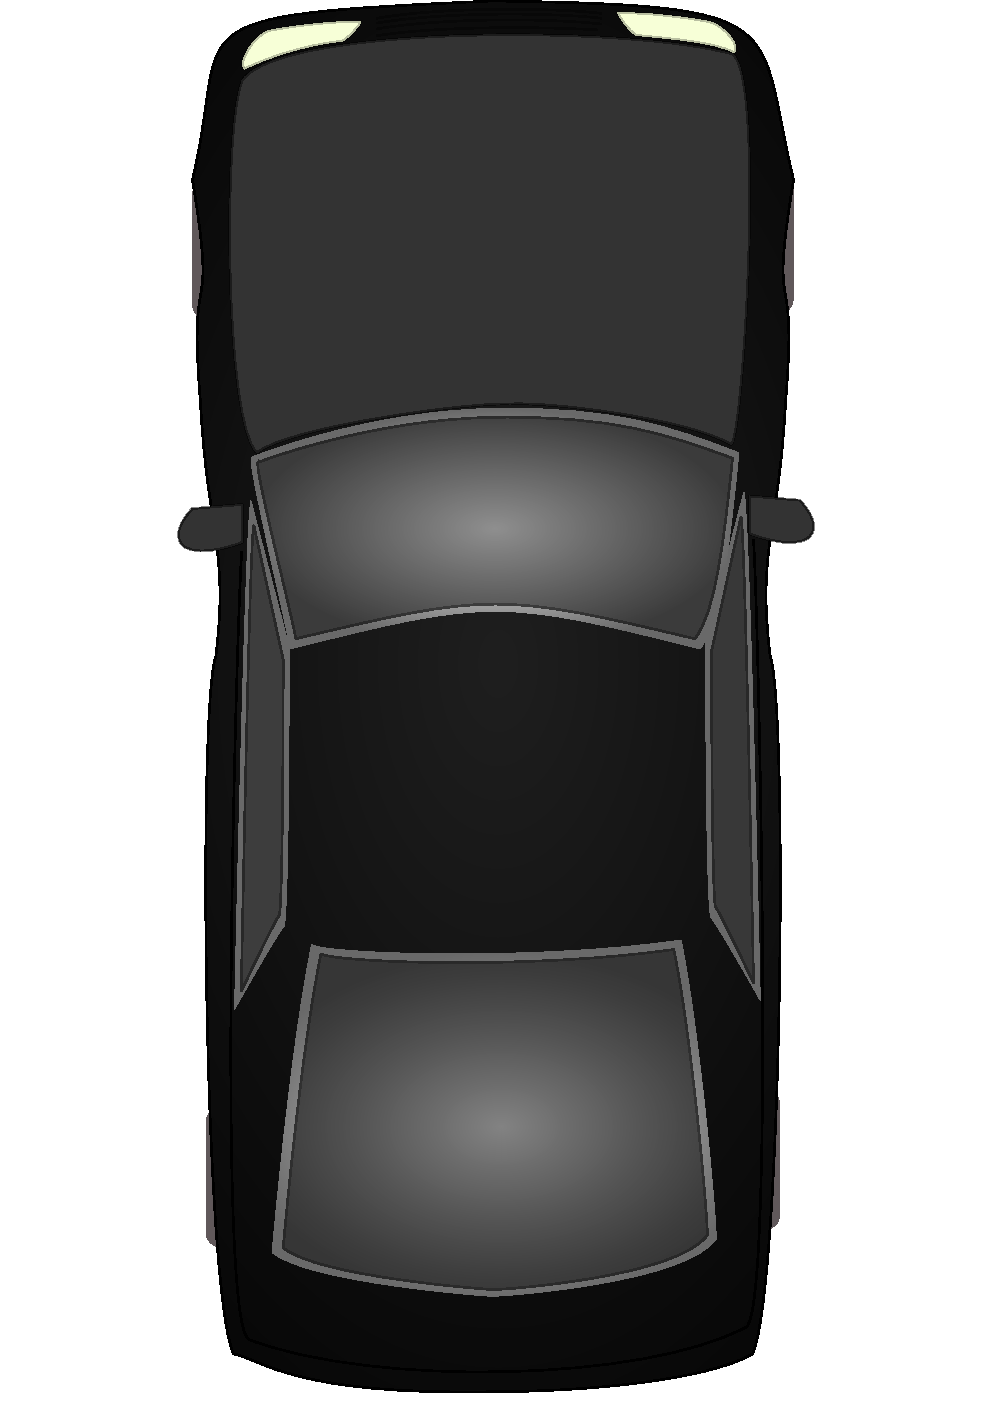
\includegraphics[width=2cm,angle=90,origin=c]{../deadlock/car-black.pdf}};
    },
    car black opposite rot/.pic={
        \node at (0,-0.25) {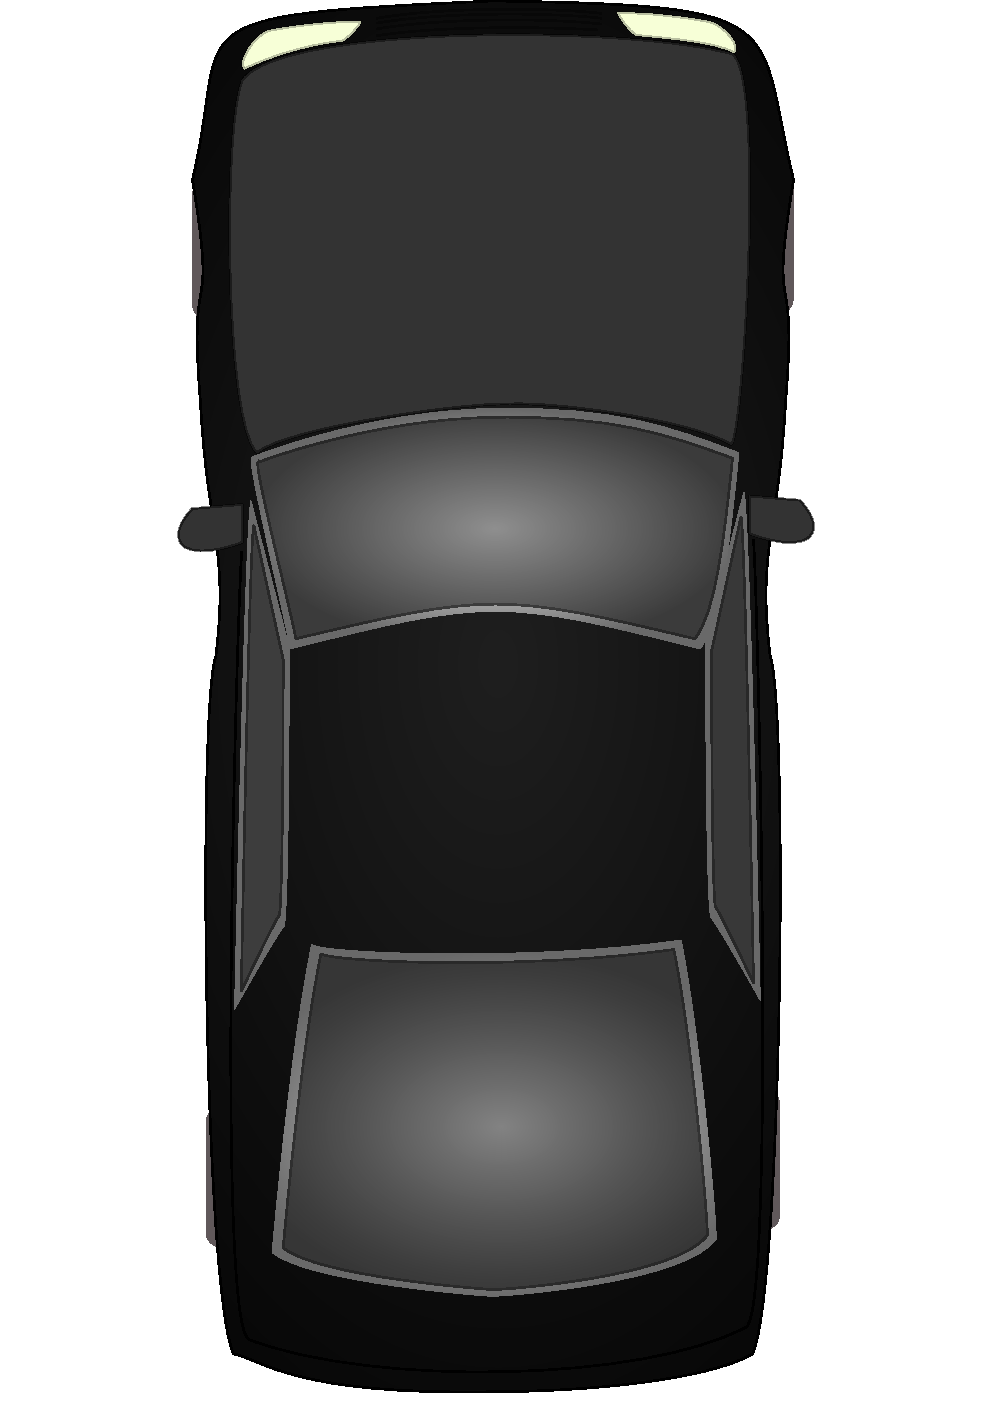
\includegraphics[width=2cm,angle=85,origin=c]{../deadlock/car-black.pdf}};
    },
    car yellow/.pic={
        \node at (0,-0.25) {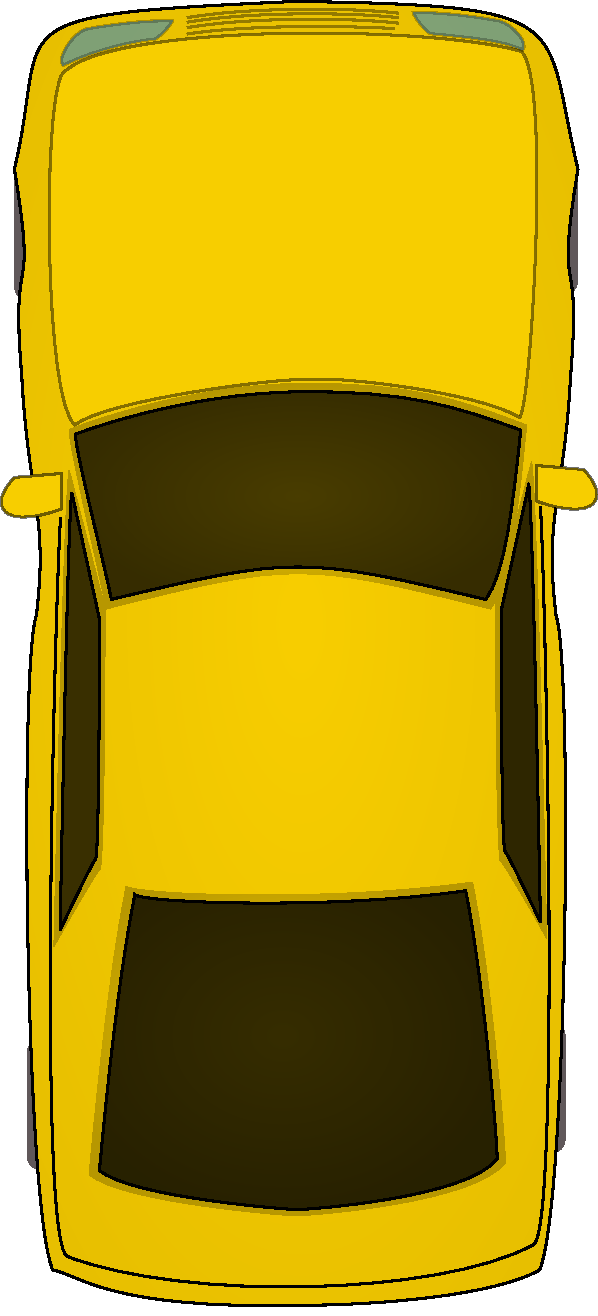
\includegraphics[width=1.25cm,angle=-90,origin=c]{../deadlock/car-yellow.pdf}};
    },
    car yellow rot/.pic={
        \node at (0,-0.25) {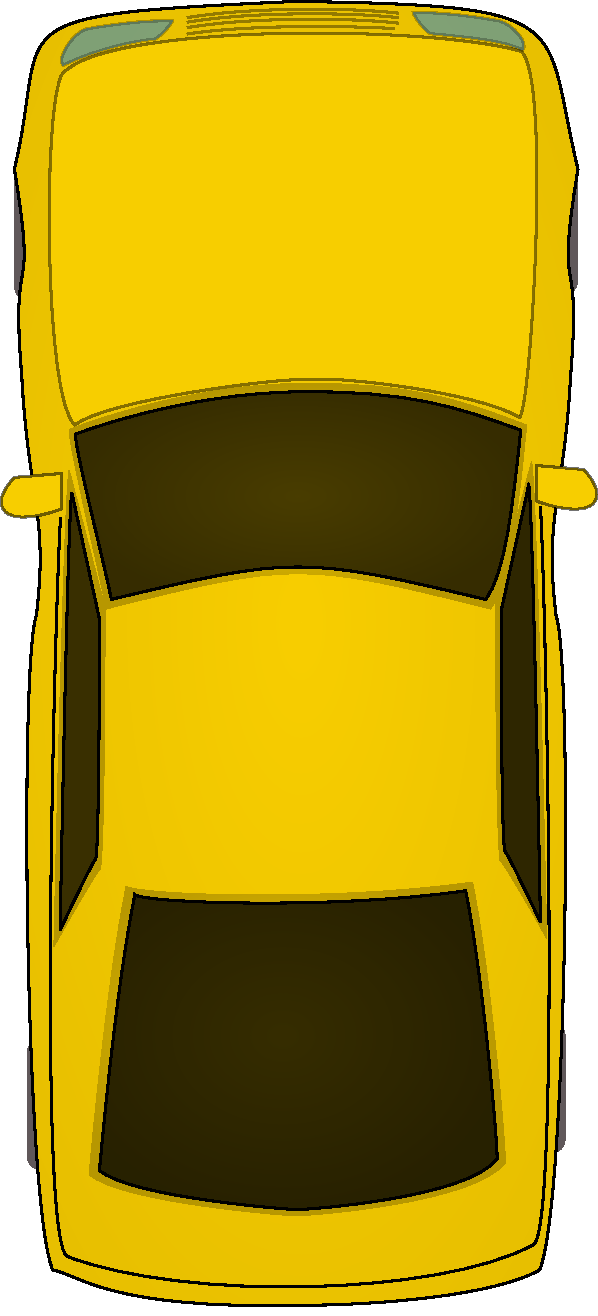
\includegraphics[width=1.25cm,angle=-100,origin=c]{../deadlock/car-yellow.pdf}};
    },
}
\draw[bridge line] (-4.5, -1) -- (-1, -1) -- (1, 0) -- (5, 0) -- (7, -1) -- (10.5, -1);
\draw[bridge line] (-4.5, 3) -- (-1, 3) -- (1, 2) -- (5, 2) -- (7, 3) -- (10.5, 3);
\draw[road divide] (-4.5, 1) -- (-1.5, 1);
\draw[road divide] (7.5, 1) -- (10.5, 1);

\begin{visibleenv}<1-2>
\path[overlay] (-3, 2) pic{car yellow};
\path[overlay] (9.5, 0) pic{car black opposite};
\end{visibleenv}

\begin{pgfonlayer}{bg}
\begin{visibleenv}<2>
\path[fill=yellow!60!black!20] (-1.5, 1) -- (-1.5, 3) -- (-1, 3) -- (1, 2) -- (2.5, 2) -- (2.5, 0) -- (1, 0) -- (-1, 1) -- cycle;
\end{visibleenv}
\begin{visibleenv}<2>
\path[fill=black!30] (8.0, 1) -- (8, -1) -- (7, -1) -- (5, 0) -- (4, 0) -- (4, 2) -- (5, 2) -- (7, 1) -- cycle;
\end{visibleenv}
\end{pgfonlayer}

\begin{visibleenv}<3-4>
\path[overlay] (1, 1.2) pic{car yellow rot};
\path[overlay] (5, 1) pic{car black opposite rot};
\end{visibleenv}

\end{tikzpicture}
\end{frame}


\subsection{with locks}
\usetikzlibrary{matrix}

\begin{frame}[fragile,label=moveFileDeadlock]{moving two files}
\begin{lstlisting}[language=C++,style=smaller]
struct Dir {
  mutex_t lock; map<string, DirEntry> entries;
};
void MoveFile(Dir *from_dir, Dir *to_dir, string filename) {
  mutex_lock(&from_dir->lock);
  mutex_lock(&to_dir->lock);
    
  to_dir->entries[filename] = from_dir->entries[filename];
  from_dir->entries.erase(filename);

  mutex_unlock(&to_dir->lock);
  mutex_unlock(&from_dir->lock);
}
\end{lstlisting}
Thread 1: \texttt{MoveFile(A, B, "foo")} \\
Thread 2: \texttt{MoveFile(B, A, "bar")} 
\end{frame}

\begin{frame}[fragile,label=moveFileNoDeadlockTimeline1]{moving two files: lucky timeline (1)}
\begin{tikzpicture}
\tikzset{
  timeline/.style={
    tight matrix no line,
    ampersand replacement=\Q,
    nodes={text width=7cm,
      minimum height=0.6cm,
        font=\small\tt\lstset{language=C++,style=small},
        },
    column sep=1cm,
    row 1/.style={nodes={font=\bfseries,align=center}},
    row 2/.style={nodes={font=\bfseries\tt}},
  },
  waiting/.style={text=black!40},
}
\matrix[timeline] (timeline) {
  Thread 1 \Q Thread 2 \\
  MoveFile(A, B, "foo") \Q MoveFile(B, A, "bar") \\
  {lock(\&A->lock);} \\
  {lock(\&B->lock);} \\
  {\normalfont (do move)} \\
  {unlock(\&B->lock);} \\
  {unlock(\&A->lock);} \\
  \Q {lock(\&B->lock);} \\
  \Q {lock(\&A->lock);} \\
  \Q {\normalfont (do move)} \\
  \Q {unlock(\&B->lock);} \\
  \Q {unlock(\&A->lock);} \\
};
\draw[very thick] (timeline-2-1.south west) -- (timeline-2-2.south east);
\end{tikzpicture}
\end{frame}

\begin{frame}[fragile,label=moveFileNoDeadlockTimeline2]{moving two files: lucky timeline (2)}
\begin{tikzpicture}
\tikzset{
  timeline/.style={
    tight matrix no line,
    ampersand replacement=\Q,
    nodes={text width=7cm,
      minimum height=0.6cm,
        font=\small\tt\lstset{language=C++,style=small},
        },
    column sep=1cm,
    row 1/.style={nodes={font=\bfseries,align=center}},
    row 2/.style={nodes={font=\bfseries\tt}},
  },
  waiting/.style={text=black!40},
}
\matrix[timeline] (timeline) {
  Thread 1 \Q Thread 2 \\
  MoveFile(A, B, "foo") \Q MoveFile(B, A, "bar") \\
  {lock(\&A->lock);} \Q \\
  {lock(\&B->lock);} \Q \\
  \Q |[waiting]| {lock(\&B->lock\ldots} \\
  {\normalfont (do move)} \Q |[waiting]|  {\normalfont (waiting for B lock)} \\
  {unlock(\&B->lock);} \\
  \Q {lock(\&B->lock);} \\
  \Q |[waiting]| {lock(\&A->lock\ldots} \\
  {unlock(\&A->lock);} \\
  \Q {lock(\&A->lock);} \\
  \Q {\normalfont (do move)} \\
  \Q {unlock(\&A->lock);} \\
  \Q {unlock(\&B->lock);} \\
};
\draw[very thick] (timeline-2-1.south west) -- (timeline-2-2.south east);
\end{tikzpicture}
\end{frame}

\begin{frame}[fragile,label=moveFileDeadlockTimeline]{moving two files: unlucky timeline}
\begin{tikzpicture}
\tikzset{
  timeline/.style={
    tight matrix no line,
    ampersand replacement=\Q,
    nodes={text width=7cm,
      minimum height=0.6cm,
        font=\small\tt\lstset{language=C++,style=small},
        },
    column sep=1cm,
    row 1/.style={nodes={font=\bfseries,align=center}},
    row 2/.style={nodes={font=\bfseries\tt}},
  },
  waiting/.style={text=black!40},
}
\matrix[timeline] (timeline) {
  Thread 1 \Q Thread 2 \\
  MoveFile(A, B, "foo") \Q MoveFile(B, A, "bar") \\
  {lock(\&A->lock);} \Q \\
  \Q {lock(\&B->lock);} \\
  {lock(\&B->lock\ldots \normalfont{ \myemph{stalled}}} \Q \\
  |[waiting]| \normalfont (waiting for lock on B) \Q {lock(\&A->lock\ldots \normalfont{ \myemph{stalled}}} \\
  |[waiting]| \normalfont (waiting for lock on B) \Q |[waiting]| \normalfont (waiting for lock on A) \\
  ~ \Q ~ \\
  \normalfont{\sout{(do move)}{ }\myemph{unreachable}} \Q \normalfont{\sout{(do move)}{ }\myemph{unreachable}} \\
  \sout{unlock(\&B->lock);}\normalfont{ \myemph{unreachable}} \Q \sout{unlock(\&A->lock);} \normalfont{ \myemph{unreachable}} \\
  \sout{unlock(\&A->lock);}\normalfont{ \myemph{unreachable}} \Q\sout{unlock(\&B->lock);} \normalfont{ \myemph{unreachable}} \\
};
\draw[very thick] (timeline-2-1.south west) -- (timeline-2-2.south east);
\begin{visibleenv}<1|handout:0>
\fill[white] (timeline-5-1.north west) rectangle (timeline.south east);
\end{visibleenv}
\begin{visibleenv}<2|handout:0>
\fill[white] (timeline-8-1.north west) rectangle (timeline.south east);
\end{visibleenv}
\begin{visibleenv}<4->
\node[anchor=north,align=center] at ([yshift=-.5cm]timeline.south) {
Thread 1 holds A lock, waiting for Thread 2 to release B lock \\
Thread 2 holds B lock, waiting for Thread 1 to release A lock 
};
\end{visibleenv}
\end{tikzpicture}
\end{frame}

\usetikzlibrary{arrows.meta,shapes.geometric}
\tikzset{
    >=Latex,
    resource/.style={draw,rectangle,very thick,align=center},
    resource m/.style={draw,rectangle,very thick,align=center,row sep=2mm},
    resource circle/.style={circle,fill=black,inner sep=0mm,minimum width=2.5mm},
    thread/.style={draw,ellipse,very thick,align=center},
    dependency/.style={draw,ultra thick,->},
    dependency future/.style={dependency,dotted},
    dependency reason/.style={align=center},
}

\begin{frame}{moving two files: dependencies}
\begin{tikzpicture}
\node[resource] (directory A) {
    directory B 
};
\node[resource] (directory B) at ([yshift=-6cm]directory A) {
    directory A
};
\node[thread] (thread one) at ([xshift=-4cm,yshift=-3cm]directory A) {
  thread 1
};
\node[thread] (thread two) at ([xshift=4cm,yshift=-3cm]directory A) {
  thread 2
};

\path[dependency] (thread one.north) ..  controls ([yshift=2cm]thread one.north) .. (directory A.west)
    node[midway,dependency reason,left] {
      waiting for lock
    };
\path[dependency] (thread two.south) ..  controls ([yshift=-2cm]thread two.south) .. (directory B.east)
    node[midway,dependency reason,right] {
      waiting for lock
    };
\path[dependency future] (directory A.east) .. controls ([yshift=2cm]thread two.north) .. (thread two.north)
    node[midway,dependency reason,right] {
      lock held by
    };
\path[dependency future] (directory B.west) .. controls ([yshift=-2cm]thread one.south) .. (thread one.south)
    node[midway,dependency reason,left] {
      lock held by
    };
\end{tikzpicture}
\end{frame}

\begin{frame}{moving three files: dependencies}
\begin{tikzpicture}
\node[resource] (directory A) {
    directory B 
};
\node[resource] (directory B) at ([yshift=-4cm,xshift=4cm]directory A) {
    directory C
};
\node[resource] (directory C) at ([yshift=-4cm,xshift=-4cm]directory A) {
    directory A
};
\node[thread] (thread one) at ([xshift=-4cm,yshift=-1.5cm]directory A) {
  thread 1
};
\node[thread] (thread two) at ([xshift=4cm,yshift=-1.5cm]directory A) {
  thread 2
};
\node[thread] (thread three) at ([yshift=-6cm]directory A) {
  thread 3
};

\path[dependency] (thread one.north) ..  controls ([yshift=1cm]thread one.north) .. (directory A.west)
    node[midway,dependency reason,left] {
      waiting for lock
    };
\path[dependency] (thread two.south) ..  controls ([yshift=-1cm]thread two.south) .. (directory B.north)
    node[midway,dependency reason,right] {
      waiting for lock
    };
\path[dependency] (thread three.west) ..  controls ([yshift=-1cm]directory C.south) .. (directory C.south)
    node[midway,dependency reason,below left] {
      waiting for lock
    };
\path[dependency future] (directory A.east) .. controls ([yshift=1cm]thread two.north) .. (thread two.north)
    node[midway,dependency reason,right] {
      lock held by
    };
\path[dependency future] (directory B.south) .. controls ([xshift=2cm]thread three.east) .. (thread three.east)
    node[midway,dependency reason,below right] {
      lock held by
    };
\path[dependency future] (directory C.north) .. controls ([yshift=-1cm]thread one.south) .. (thread one.south)
    node[midway,dependency reason,left] {
      lock held by
    };
\end{tikzpicture}
\end{frame}

\begin{frame}[fragile,label=moveFileDeadlockTimeline2]{moving three files: unlucky timeline}
\begin{tikzpicture}
\tikzset{
  timeline/.style={
    tight matrix no line,
    ampersand replacement=\Q,
    nodes={text width=4.5cm,
      minimum height=0.6cm,
        font=\fontsize{9.5}{10.5}\selectfont\tt\lstset{language=C++,style=small},
        },
    column sep=0.25cm,
    row 1/.style={nodes={font=\fontsize{10}{11}\selectfont\bfseries,align=center}},
    row 2/.style={nodes={font=\fontsize{10}{11}\selectfont\bfseries\tt}},
  waiting/.style={text=black!40},
  },
}
\matrix[timeline] (timeline) {
  Thread 1 \Q Thread 2 \Q Thread 3\\
  MoveFile(A, B, "foo") \Q MoveFile(B, C, "bar") \Q MoveFile(C, A, "quux") \\
  {lock(\&A->lock);} \Q ~ \Q ~\\
  \Q {lock(\&B->lock);} \\
  \Q \Q {lock(\&C->lock);} \\
  {lock(\&B->lock\ldots}{ }\normalfont{\myemph{stalled}} \Q \\
  \Q {lock(\&C->lock\ldots}{ }\normalfont{\myemph{stalled}} \\
  \Q \Q {lock(\&A->lock\ldots}{ }\normalfont{\myemph{stalled}} \\
};
\begin{scope}[red!70!black]
\draw[dashed,-Latex,thick,in=-90] ([xshift=-.75cm]timeline-6-1.east) to (timeline-4-2.south);
\draw[dashed,-Latex,thick,in=-90] ([xshift=-.75cm]timeline-7-2.east) to (timeline-5-3.south);
\draw[dashed,-Latex,thick] ([xshift=-.75cm]timeline-8-3.east) to[out=0,in=0] (timeline-3-3.center) to ([xshift=-1cm]timeline-3-1.east);
\end{scope}
\end{tikzpicture}
\end{frame}


\subsection{with memory}
\begin{frame}{deadlock with free space}
\begin{tikzpicture}
\tikzset{
  timeline/.style={
    tight matrix no line,
    ampersand replacement=\Q,
    nodes={text width=7cm,
      minimum height=0.6cm,
        font=\small\tt\lstset{language=C++,style=small},
        },
    column sep=1cm,
    row 1/.style={nodes={font=\bfseries,align=center}},
  },
  waiting/.style={text=black!40},
}
\matrix[timeline] (timeline) {
  Thread 1 \Q Thread 2 \\
  AllocateOrWaitFor(1 MB) \Q AllocateOrWaitFor(1 MB) \\
  AllocateOrWaitFor(1 MB) \Q AllocateOrWaitFor(1 MB) \\
  (do calculation) \Q (do calculation) \\
  Free(1 MB) \Q Free(1 MB) \\
  Free(1 MB) \Q Free(1 MB) \\
};
\node[anchor=north,align=center] at (timeline.south) { 
  2 MB of space --- deadlock possible with unlucky order
};
\end{tikzpicture}
\end{frame}

\begin{frame}{deadlock with free space (unlucky case)}
\begin{tikzpicture}
\tikzset{
  timeline/.style={
    tight matrix no line,
    ampersand replacement=\Q,
    nodes={text width=7cm,
      minimum height=0.6cm,
        font=\small\tt\lstset{language=C++,style=small},
        },
    column sep=1cm,
    row 1/.style={nodes={font=\bfseries,align=center}},
  },
  waiting/.style={text=black!40},
}
\matrix[timeline] (timeline) {
  Thread 1 \Q Thread 2 \\
  AllocateOrWaitFor(1 MB) \\
  \Q  AllocateOrWaitFor(1 MB) \\
  AllocateOrWaitFor(1 MB\ldots{ }\normalfont{\myemph{stalled}} \\
  \Q AllocateOrWaitFor(1 MB\ldots{ }\normalfont{\myemph{stalled}} \\
};
\node[anchor=north,align=center] at (timeline.south) { 

};
\end{tikzpicture}
\end{frame}

\begin{frame}[fragile,label=freeSpaceDepend]{free space: dependency graph}
\begin{tikzpicture}
    \newcommand{\mycircle}[1]{
        \node[resource circle] (#1) {};
    }
    \matrix[resource,row sep=2mm,label={[align=left,xshift=-1cm]north east:{memory in \\2 (1MB) units}}] (resource A) {
    \mycircle{A one} \\
    \mycircle{A two} \\
};
\node[thread] (thread one) at ([xshift=-3cm,yshift=-3cm]resource A) {
  thread 1
};
\node[thread] (thread two) at ([xshift=3cm,yshift=-3cm]resource A) {
  thread 2
};
    \path[dependency future] (A one.west) .. controls ([xshift=-1cm]A one.west) .. (thread one.north)
        node[pos=0.8,above] {allocated};
    \path[dependency future] (A two.east) .. controls ([xshift=1cm]A two.east) .. (thread two.north);
    \path[dependency] (thread one.east) .. controls ([xshift=1cm]thread one.east) .. (resource A.south)
        node[midway,below=.5cm,xshift=1cm] {waiting for};
    \path[dependency] (thread two.west) .. controls ([xshift=-1cm]thread two.west) .. (resource A.south);
\end{tikzpicture}
\end{frame}

\begin{frame}{deadlock with free space (lucky case)}
\begin{tikzpicture}
\tikzset{
  timeline/.style={
    tight matrix no line,
    ampersand replacement=\Q,
    nodes={text width=7cm,
      minimum height=0.6cm,
        font=\small\tt\lstset{language=C++,style=small},
        },
    column sep=1cm,
    row 1/.style={nodes={font=\bfseries,align=center}},
  },
  waiting/.style={text=black!40},
}
\matrix[timeline] (timeline) {
  Thread 1 \Q Thread 2 \\
  AllocateOrWaitFor(1 MB) \\
  AllocateOrWaitFor(1 MB) \\
  (do calculation) \\
  Free(1 MB); \\ 
  Free(1 MB); \\
  \Q AllocateOrWaitFor(1 MB) \\
  \Q AllocateOrWaitFor(1 MB) \\
  \Q (do calculation) \\
  \Q Free(1 MB); \\ 
  \Q Free(1 MB); \\
};
\end{tikzpicture}
\end{frame}

 
\section{deadlock definition}

\subsection{short intuition}

\begin{frame}{deadlock}
\begin{itemize}
\item deadlock --- circular waiting for \myemph<2>{resources}
\vspace{.5cm}
\item resource = something needed by a thread to do work
  \begin{itemize}
  \item locks
  \item CPU time
  \item disk space
  \item memory
  \item \ldots
  \end{itemize}
\item often non-deterministic in practice
\item most common example: \myemph{when acquiring multiple locks}
\end{itemize}
\end{frame}

\begin{frame}{deadlock versus starvation}
\begin{itemize}
\item starvation: one+ unlucky (no progress), 
                  one+ lucky (yes progress)
    \begin{itemize}
    \item example: low priority threads versus high-priority threads
    \end{itemize}
\item deadlock: no one involved in deadlock makes progress
\vspace{.5cm}
\item<2-> starvation: once starvation happens, taking turns will resolve
    \begin{itemize}
    \item low priority thread just needed a chance\ldots
    \end{itemize}
\item<2-> deadlock: once it happens, taking turns won't fix
\end{itemize}
\end{frame}


\subsection{conditions for deadlock}

\begin{frame}{deadlock requirements}
\begin{itemize}
\item \textbf{mutual exclusion}
    \begin{itemize}
    \item one thread at a time can use a resource
    \end{itemize}
\item \textbf{hold and wait}
  \begin{itemize}
  \item thread holding a resources waits to acquire \textit{another} resource
  \end{itemize}
\item \textbf{no preemption of resources}
    \begin{itemize}
    \item resources are only released voluntarily
    \item thread trying to acquire resources can't `steal'
    \end{itemize}
\item \textbf{circular wait}
    \begin{itemize}
    \item there exists a set $\{T_1,\ldots,T_n\}$ of waiting threads such that
        \begin{itemize}
        \item $T_1$ is waiting for a resource held by $T_2$
        \item $T_2$ is waiting for a resource held by $T_3$
        \item \ldots
        \item $T_n$ is waiting for a resource held by $T_1$
        \end{itemize}
    \end{itemize}
\end{itemize}
\end{frame}


\section{exercise}

\begin{frame}[fragile,label=isDeadlockP]{how is deadlock possible?}
Given list: A, B, C, D, E
\begin{lstlisting}[style=size10]
RemoveNode(LinkedListNode *node) {
    pthread_mutex_lock(&node->lock);
    pthread_mutex_lock(&node->prev->lock);
    pthread_mutex_lock(&node->next->lock);
    node->next->prev = node->prev; node->prev->next = node->next;
    pthread_mutex_unlock(&node->next->lock); pthread_mutex_unlock(&node->prev->lock);
    pthread_mutex_unlock(&node->lock);
}
\end{lstlisting}
Which of these (all run in parallel) can deadlock? \\
\begin{tabular}{l} 
A. RemoveNode(B) and RemoveNode(C) \\
B. RemoveNode(B) and RemoveNode(D) \\
C. RemoveNode(B) and RemoveNode(C) and RemoveNode(D) \\
D. A and C \hspace{3cm} E. B and C \\
F. all of the above \hspace{1cm} G. none of the above \\
\end{tabular}
\end{frame}

\begin{frame}<0>[label=isDeadlockPTimeline1]{how is deadlock --- solution}
\begin{tabular}{l|l}
Remove B & Remove C \\
lock B & lock C \\
lock A (prev) & wait to lock B (prev) \\
wait to lock C (next) &
\end{tabular}
\hrule
With B and D --- only overlap in in node C --- no circular wait possible
\end{frame}

\iftoggle{heldback}{}{\againframe<1>{isDeadlockPTimeline1}}


\section{deadlock prevention}

\subsection{techniques overview}

\usetikzlibrary{matrix,positioning,shapes.callouts}

\begin{frame}<0>[label=deadlockPrevent]{deadlock prevention techniques}
\begin{tikzpicture}
\matrix[
  tight matrix no line,
  column 1/.style={nodes={text width=10cm,align=left}},
  column 2/.style={nodes={text width=5cm}},
  row sep=.5cm,
] {
{%
  \textbf{\myemph<2>{infinite resources}} \\
  \hspace{1cm}or at least enough that never run out
} \& {no \textit{mutual exclusion}} \\
{%
  \textbf{\myemph<3>{no shared resources}}
} \& {no \textit{mutual exclusion}} \\
|[alias=no wait]| {%
  \textbf{\myemph<4,7,8>{no waiting}} \\
\hspace{1cm} ``\myemph<4,8>{busy signal}'' --- \myemph<4,8>{abort and (maybe) retry} \\
\hspace{1cm} \myemph<7>{revoke/preempt resources}
} \& {no \textit{hold and wait}/\\\textit{preemption}} \\
{%
  acquire resources in \textbf{\myemph<5>{consistent order}}
} \& {no \textit{circular wait}} \\
{%
  request \textbf{\myemph<6>{all resources at once}}
} \& {no \textit{hold and wait}} \\
};
\begin{visibleenv}<4>
\coordinate (abort retry) at ([xshift=-3cm,yshift=-.7cm]no wait.north east);
\node[my callout2=abort retry,anchor=south east,align=left,font=\small] at ([xshift=5cm,yshift=.9cm]abort retry) {
    memory allocation: malloc() fails rather than waiting (no deadlock) \\
    locks: \texttt{pthread\_mutex\_trylock} fails rather than waiting \\
    problem: retry how many times? \myemph{no bound on number of tries needed} \\
    \ldots
};
\end{visibleenv}
\begin{visibleenv}<7>
\coordinate (revoke) at ([xshift=-3cm,yshift=-1cm]no wait.north east);
\node[my callout2=abort retry,anchor=south east,align=left,font=\small] at ([xshift=5cm,yshift=.5cm]revoke) {
    requires some way to undo partial changes to avoid errors \\
    common approach for databases \\
    \ldots
};
\end{visibleenv}
\end{tikzpicture}
\end{frame}


% FIXME: cut down?

\againframe<1>{deadlockPrevent}

\againframe<2>{deadlockPrevent} % infinite resources

\againframe<3>{deadlockPrevent} % no shared resources

\subsection{example: no waiting}

\againframe<4>{deadlockPrevent} % no waiting (abort and retry)

\subsection{revocable locks}

\againframe<7>{deadlockPrevent} % no waiting (revoke)

\subsection{example: consistent order}

\againframe<5>{deadlockPrevent}

\usetikzlibrary{matrix}

\begin{frame}[fragile,label=moveFileOrdering]{acquiring locks in consistent order (1)}
\begin{lstlisting}[
    language=C++,
    style=small,
    moredelim={**[is][\btHL<2|handout:2>]{@2}{2@}},
]
MoveFile(Dir* from_dir, Dir* to_dir, string filename) {
  if @2(from_dir->path < to_dir->path)2@ {
    lock(&from_dir->lock);
    lock(&to_dir->lock);
  } else {
    lock(&to_dir->lock);
    lock(&from_dir->lock);
  }
  ...
}
\end{lstlisting}
\begin{tikzpicture}[overlay,remember picture]
\begin{visibleenv}<2>
\node[anchor=south,draw=red,thick,align=center] at ([yshift=1cm]current page.south) {
  any ordering will do \\
  e.g. compare pointers
};
\end{visibleenv}
\end{tikzpicture}
\end{frame}

\begin{frame}[fragile,label=linuxOrdering]{acquiring locks in consistent order (2)}
\begin{itemize}
\item often by convention, e.g. Linux kernel comments:
\end{itemize}
\begin{lstlisting}[language=C++,style=smaller]
/*
 * ...
 * Lock order:
 *	contex.ldt_usr_sem
 *	  mmap_sem
 *	    context.lock
 */
\end{lstlisting}
\hrule
\begin{lstlisting}[language=C++,style=smaller]
/*
 * ...
 * Lock order:
 *   1. slab_mutex (Global Mutex)
 *   2. node->list_lock
 *   3. slab_lock(page) (Only on some arches and for debugging)
 * ...
 */
 \end{lstlisting}
\end{frame}




\againframe<6>{deadlockPrevent}

\subsection{deadlock detection}


\begin{frame}{deadlock detection}
    \begin{itemize}
    \item why? debugging or fix deadlock by aborting operations
    \item idea: search for cyclic dependencies
    \end{itemize}
\end{frame}

\begin{frame}[fragile,label=detectLocks]{detecting deadlocks on locks}
    \begin{itemize}
    \item let's say I want to detect deadlocks that only involve mutexes
        \begin{itemize}
        \item goal: help programmers debug deadlocks
        \end{itemize}
    \item \ldots by modifying my threading library:
    \end{itemize}
\begin{lstlisting}[language=C++,style=smaller]
struct Thread {
    ... /* stuff for implementing thread */
    /* what extra fields go here? */


};

struct Mutex {
    ... /* stuff for implementing mutex */
    /* what extra fields go here? */


};
\end{lstlisting}
\end{frame}

\begin{frame}{deadlock detection}
    \begin{itemize}
    \item why? debugging or fix deadlock by aborting operations
    \item idea: search for cyclic dependencies
    \item need:
        \begin{itemize}
        \item list of all contended resources
        \item what thread is waiting for what?
        \item what thread `owns' what?
        \end{itemize}
    \end{itemize}
\end{frame}




\subsubsection{problem with divisible resources?}
\begin{frame}{aside: divisible resources}
    \begin{itemize}
    \item deadlock is possible with divislbe resources like memory,\ldots
    \item example: suppose 6MB of RAM for threads total:
        \begin{itemize}
        \item thread 1 has 2MB allocated, waiting for 2MB
        \item thread 2 has 2MB allocated, waiting for 2MB
        \item thread 3 has 1MB allocated, waiting for keypress
        \end{itemize}
    \item cycle: thread 1 waiting on memory owned by thread 2?
    \item not a deadlock --- thread 3 can still finish
        \begin{itemize}
        \item and after it does, thread 1 or 2 can finish
        \end{itemize}
    \item<2-> \ldots but would be deadlock
        \begin{itemize}
            \item \ldots if thread 3 waiting lock held by thread 1
            \item \ldots with 5MB of RAM
        \end{itemize}
    \end{itemize}
\end{frame}

\begin{frame}[fragile,label=divisibleGraphNotDead]{divisible resources: not deadlock}
\begin{tikzpicture}
    \newcommand{\mycircle}[1]{
        \node[resource circle] (#1) {};
    }
    \matrix[resource,row sep=2mm,label={[align=left,xshift=-1cm]north east:{memory in \\6 (1MB) units}}] (resource A) {
    \mycircle{A one} \\
    \mycircle{A two} \\
    \mycircle{A three} \\
    \mycircle{A four} \\
    \mycircle{A five} \\
    \mycircle{A six} \\
};
\node[thread] (thread one) at ([xshift=-3cm,yshift=-3cm]resource A) {
  thread 1
};
\node[thread] (thread two) at ([xshift=3cm,yshift=-3cm]resource A) {
  thread 2
};
\node[thread] (thread three) at ([xshift=-2cm, yshift=3cm]resource A) {
    thread 3
};
\begin{visibleenv}<4->
    \path[alt=<4>{red},dependency future,alt=<5->{opacity=0.1}] (A one.west) ..  controls ([yshift=2cm]thread one.north) .. (thread one.north);
    \path[alt=<4>{red},dependency future,alt=<5->{opacity=0.1}] (A two.west) ..  controls ([yshift=2cm]thread one.north) .. (thread one.north);
\end{visibleenv}
\begin{visibleenv}<6->
    \path[alt=<6>{red},dependency future,alt=<7->{opacity=0.1}] (A one.east) ..  controls ([yshift=2cm]thread two.north) .. (thread two.north);
    \path[alt=<6>{red},dependency future,alt=<7->{opacity=0.1}] (A two.east) ..  controls ([yshift=2cm]thread two.north) .. (thread two.north);
\end{visibleenv}
    \path[dependency future,alt=<3->{opacity=0.2}] (A one.west) .. controls ([xshift=-1cm]A one.west) .. (thread three.south)
    node[pos=0.8,dependency reason,font=\small,fill=white] {
        owns 
    };

    \path[dependency,alt=<4->{invisible}] (thread one.east) ..  controls ([xshift=1cm]thread one.east) .. (resource A.south)
    node[alt=<4->{opacity=1.0},alt=<6->{opacity=0},midway,dependency reason,font=\small,below,xshift=1cm] {
      waiting for \\ 2MB
    };
    \path[dependency future,alt=<5->{invisible}] (A four.west) ..  controls ([yshift=2cm]thread one.north) .. (thread one.north);
    \path[dependency future,alt=<5->{invisible}] (A three.west) ..  controls ([yshift=2cm]thread one.north) .. (thread one.north)
    node[pos=0.8,dependency reason,font=\small,fill=white] {
        owns 
    };
    \path[dependency,alt=<6->{invisible}] (thread two.west) ..  controls ([xshift=-1cm]thread two.west) .. (resource A.south)

    ;
\path[dependency future,alt=<7->{opacity=0.1}] (A six.east) .. controls ([yshift=2cm]thread two.north) .. (thread two.north);
\path[dependency future,alt=<7->{opacity=0.1}] (A five.east) .. controls ([yshift=2cm]thread two.north) .. (thread two.north)
    node[midway,dependency reason,font=\small,fill=white] {
        owns 
    }
    ;
\begin{visibleenv}<2->
    \node[draw,very thick,anchor=west,align=left] at ([xshift=4cm,yshift=0cm]resource A) {
        not deadlock: \\
        \myemph<3>{thread 3 finishes} \\
        \myemph<4>{then thread 1 can get memory} \\
        \myemph<5>{then thread 1 finishes} \\
        \myemph<6>{then thread 2 can get resources} \\
        \myemph<7>{then thread 2 can finish}
    };
\end{visibleenv}
\end{tikzpicture}
\end{frame}

\begin{frame}[fragile,label=divisibleGraphIsDeadLock]{divisible resources: is deadlock}
\begin{tikzpicture}
    \newcommand{\mycircle}[1]{
        \node[resource circle] (#1) {};
    }
    \matrix[resource,row sep=2mm,label={[align=left,xshift=-1cm]north east:{memory in \\6 (1MB) units}}] (resource A) {
    \mycircle{A one} \\
    \mycircle{A two} \\
    \mycircle{A three} \\
    \mycircle{A four} \\
    \mycircle{A five} \\
    \mycircle{A six} \\
};
\node[thread] (thread one) at ([xshift=-3cm,yshift=-3cm]resource A) {
  thread 1
};
\node[thread] (thread two) at ([xshift=3cm,yshift=-3cm]resource A) {
  thread 2
};
\node[thread] (thread three) at ([xshift=-2cm, yshift=3cm]resource A) {
    thread 3
};

    \path[dependency future] (A one.west) .. controls ([xshift=-1cm]A one.west) .. (thread three.south)
    ;

    \path[dependency,double] (thread one.east) ..  controls ([xshift=1cm]thread one.east) .. (resource A.south)
    node[midway,dependency reason,font=\small,below,xshift=1cm] {
      waiting for \\ 2MB
    };
    \path[dependency future] (A four.west) ..  controls ([yshift=2cm]thread one.north) .. (thread one.north);
    \path[dependency future] (A three.west) ..  controls ([yshift=2cm]thread one.north) .. (thread one.north)
    node[pos=0.8,dependency reason,font=\small,fill=white] {
        owns 
    };
    \path[dependency,double] (thread two.west) ..  controls ([xshift=-1cm]thread two.west) .. (resource A.south)
    ;
\path[dependency future] (A six.east) .. controls ([yshift=2cm]thread two.north) .. (thread two.north);
\path[dependency future] (A five.east) .. controls ([yshift=2cm]thread two.north) .. (thread two.north)
    node[midway,dependency reason,font=\small,fill=white] {
        owns 
    };
    \node[resource,red] (lock) at ([xshift=-.5cm,yshift=-2cm]thread three.south) {lock};
    \path[dependency] (thread three.south) .. controls ([yshift=-1cm]thread three.south) .. (lock.north);
    \path[dependency future] (lock.south) .. controls ([xshift=-1cm,yshift=-1cm]lock.south) .. (thread one.120);
    \begin{visibleenv}<2->
    \node[draw,very thick,anchor=west,align=left] at ([xshift=4cm,yshift=0cm]resource A) {
        deadlock: \\
        thread 3 can't finish \\
        until thread 1 releases lock, but \\
        thread 1 can't finish \\
        until thread 3 releases memory
    };
    \end{visibleenv}
\end{tikzpicture}
\end{frame}



\begin{frame}[fragile,label=divisibleGraphIsDeadSpace]{divisible resources: is deadlock}
\begin{tikzpicture}
    \newcommand{\mycircle}[1]{
        \node[resource circle] (#1) {};
    }
    \matrix[resource,row sep=2mm,label={[align=left,xshift=-1cm]north east:{memory in \\\myemph{5} (1MB) units}}] (resource A) {
    \mycircle{A one} \\
    \mycircle{A two} \\
    \mycircle{A three} \\
    \mycircle{A four} \\
    \mycircle{A five} \\
};
\node[thread] (thread one) at ([xshift=-3cm,yshift=-3cm]resource A) {
  thread 1
};
\node[thread] (thread two) at ([xshift=3cm,yshift=-3cm]resource A) {
  thread 2
};
\node[thread] (thread three) at ([xshift=-2cm, yshift=3cm]resource A) {
    thread 3
};

    \path[dependency future,alt=<3->{opacity=0.2}] (A one.west) .. controls ([xshift=-1cm]A one.west) .. (thread three.south)
    node[pos=0.8,dependency reason,font=\small,fill=white] {
        owns 
    };

    \path[double,dependency] (thread one.east) ..  controls ([xshift=1cm]thread one.east) .. (resource A.south)
    node[alt=<4->{opacity=1.0},alt=<6->{opacity=0},midway,dependency reason,font=\small,below,xshift=1cm] {
      waiting for \\ 2MB
    };
    \path[dependency future] (A three.west) ..  controls ([yshift=2cm]thread one.north) .. (thread one.north);
    \path[dependency future] (A two.west) ..  controls ([yshift=2cm]thread one.north) .. (thread one.north)
    node[pos=0.8,dependency reason,font=\small,fill=white] {
        owns 
    };
    \path[double,dependency] (thread two.west) ..  controls ([xshift=-1cm]thread two.west) .. (resource A.south)
    %node[midway,dependency reason,font=\small,below,xshift=1cm] {
    %  waiting for \\ 2MB
    %};
    ;
\path[dependency future] (A five.east) .. controls ([yshift=2cm]thread two.north) .. (thread two.north);
\path[dependency future] (A four.east) .. controls ([yshift=2cm]thread two.north) .. (thread two.north)
    node[midway,dependency reason,font=\small,fill=white] {
        owns 
    };
    \begin{visibleenv}<2->
    \node[draw,very thick,anchor=west,align=left] at ([xshift=4cm,yshift=0cm]resource A) {
        reducing memory: deadlock: \\
        even after thread 3 finishes \\
        no way for thread 1+2 \\ to get what they want 
    };
    \end{visibleenv}
\end{tikzpicture}
\end{frame}

\begin{frame}{deadlock detection with divisibe resources}
    \begin{itemize}
    \item can't rely on cycles in graphs in this case
    \item alternate algorithm exists
        \begin{itemize}
        \item similar technique to how we showed no deadlock
        \end{itemize}
    \item high-level intuition: simulate what could happen
        \begin{itemize}
        \item find threads that could finish based on resources available now
        \end{itemize}
    \vspace{.5cm}
    \item full details: look up Baker's algorithm
    \end{itemize}
\end{frame}



\subsection{revokable locks}

\begin{frame}{stealing locks???}
    \begin{itemize}
    \item how do we make stealing locks possible
    \vspace{.5cm}
    \item unclean: just kill the thread
        \begin{itemize}
        \item problem: inconsistent state?
        \end{itemize}
    \item clean: have code to undo partial oepration
        \begin{itemize}
        \item some databases do this
        \end{itemize}
    \item won't go into detail in this class
    \end{itemize}
\end{frame}

\begin{frame}[fragile,label=revokeLock]{revokable locks?}
\begin{lstlisting}[language=C++,style=small]
try {
    AcquireLock();
    use shared data
} catch (LockRevokedException le) {
    undo operation hopefully?
} finally {
    ReleaseLock();
}
\end{lstlisting}
\end{frame}


\subsection{example: livelock}

\againframe<8>{deadlockPrevent} % no waiting (abort and retry)

\begin{frame}{abort and retry limits?}
\begin{itemize}
\item abort-and-retry
\item how many times will you retry?
\end{itemize}
\end{frame}

\begin{frame}[fragile,label=moveFileWithRetry]{moving two files: abort-and-retry}
\begin{lstlisting}[language=C++,style=smaller]
struct Dir {
  mutex_t lock; map<string, DirEntry> entries;
};
void MoveFile(Dir *from_dir, Dir *to_dir, string filename) {
  while (true) {
    mutex_lock(&from_dir->lock);
    if (mutex_trylock(&to_dir->lock) == LOCKED) break;
    mutex_unlock(&from_dir->lock);
  }
    
  to_dir->entries[filename] = from_dir->entries[filename];
  from_dir->entries.erase(filename);

  mutex_unlock(&to_dir->lock);
  mutex_unlock(&from_dir->lock);
}
\end{lstlisting}
Thread 1: \texttt{MoveFile(A, B, "foo")} \\
Thread 2: \texttt{MoveFile(B, A, "bar")} 
\end{frame}

\begin{frame}[fragile,label=moveFileLivelockTimeline]{moving two files: lots of bad luck?}
\begin{tikzpicture}
\tikzset{
  timeline/.style={
    tight matrix no line,
    ampersand replacement=\Q,
    nodes={text width=7cm,
      minimum height=0.6cm,
        font=\small\tt\lstset{language=C++,style=small},
        },
    column sep=1cm,
    row 1/.style={nodes={font=\bfseries,align=center}},
    row 2/.style={nodes={font=\bfseries\tt}},
  },
  waiting/.style={text=black!40},
}
\matrix[timeline] (timeline) {
  Thread 1 \Q Thread 2 \\
  MoveFile(A, B, "foo") \Q MoveFile(B, A, "bar") \\
  {lock(\&A->lock) $\rightarrow$ LOCKED} \Q \\
  \Q {lock(\&B->lock) $\rightarrow$ LOCKED} \\
  {trylock(\&B->lock) $\rightarrow$ FAILED} \Q \\
  \Q {trylock(\&A->lock) $\rightarrow$ FAILED} \\
  {unlock(\&A->lock)} \Q \\
  \Q {unlock(\&B->lock)} \\
  {lock(\&A->lock) $\rightarrow$ LOCKED} \Q \\
  \Q {lock(\&B->lock) $\rightarrow$ LOCKED} \\
  {trylock(\&B->lock) $\rightarrow$ FAILED} \Q \\
  \Q {trylock(\&A->lock) $\rightarrow$ FAILED} \\
  {unlock(\&A->lock)} \Q \\
  \Q {unlock(\&B->lock)} \\
};
\draw[very thick] (timeline-2-1.south west) -- (timeline-2-2.south east);
\end{tikzpicture}
\end{frame}

\begin{frame}{livelock}
\begin{itemize}
\item livelock: keep aborting and retrying without end
\vspace{.5cm}
\item like deadlock --- no one's making progress
    \begin{itemize}
    \item potentially forever
    \end{itemize}
\item unlike deadlock --- threads are not waiting
\end{itemize}
\end{frame}

\begin{frame}{preventing livelock}
    \begin{itemize}
    \item make schedule random --- e.g. random waiting after abort
    \item make threads run one-at-a-time if lots of aborting
    \item other ideas?
    \end{itemize}
\end{frame}




\section{monitors}

\subsection{introduction}
\usetikzlibrary{arrows.meta,calc,chains,fit,matrix}

\begin{frame}{monitors/condition variables}
\begin{itemize}
\item \myemph{locks} for mutual exclusion
\item \myemph{condition variables} for waiting for event
    \begin{itemize}
    \item operations: wait (for event); signal/broadcast (that event happened)
    \end{itemize}
\item related data structures
\vspace{.5cm}
\item \myemph{monitor} = lock + 0 or more condition variables + shared data
    \begin{itemize}
    \item Java: every object is a monitor (has instance variables, built-in lock, cond. var)
    \item pthreads: build your own: provides you locks + condition variables
    \end{itemize}
\end{itemize}
\end{frame}

\begin{frame}[fragile,label=monitorIdea]{monitor idea}
\begin{tikzpicture}
\tikzset{
    hilite red on/.style={alt=<#1>{fill=red!10}},
    hilite blue on/.style={alt=<#1>{fill=blue!10}},
    >=Latex,
    queue node/.style={draw,thick,minimum width=.6cm,minimum height=.6cm},
    queue connect/.style={draw,->,ultra thick},
}
\matrix[
    tight matrix,
    nodes={draw,thick,text width=4cm,font=\small},
    label={[font=\small]north:a monitor},
    ] (monitor) {
    |[hilite red on={2-}]| lock \\
    shared data \\
    |[hilite blue on={4-}]| condvar 1 \\
    |[hilite blue on={4-}]| condvar 2 \\
    \ldots \\
    |[minimum height=0.2mm]| {} \\
    operation1(\ldots)\\
    operation2(\ldots) \\
};
\begin{visibleenv}<2-3|handout:2>
    \node[draw=red,ultra thick,inner sep=0mm,fit=(monitor-2-1) (monitor-5-1)] {};
\end{visibleenv}
\begin{visibleenv}<2|handout:0>
    \node[red,anchor=north west,align=left] at (monitor-1-1.north east) {
            lock must be acquired \\
            before accessing \\
            any part of monitor's stuff
    };
\end{visibleenv}
\begin{visibleenv}<3->
    \begin{scope}[
        start chain=going right,
        every join/.style={queue connect},
        every node/.style={queue node,on chain,join,fill=red!10},
    ]
    \node[anchor=west] (lock queue 1) at ([xshift=1cm]monitor-1-1.east) {};
    \node (lock queue 2) {};
    \node (lock queue 3) {};
    \end{scope}
    \draw[->,dashed,ultra thick] (monitor-1-1) -- (lock queue 1);
\end{visibleenv}
\begin{visibleenv}<3->
    \node[anchor=west,align=left,text=red!20!black] at ([xshift=0cm]lock queue 3.east) {
        threads waiting for lock
    };
\end{visibleenv}
\begin{visibleenv}<4->
    \begin{scope}[
        start chain=going right,
        every join/.style={queue connect},
        every node/.style={queue node,on chain,join,fill=blue!10},
    ]
    \node[anchor=west] (condvar 1 queue 1) at ([xshift=1cm,yshift=-1cm]monitor-3-1.east) {};
    \node (condvar 1 queue 2) {};
    \node (condvar 1 queue 3) {};
    \end{scope}
    \draw[->,dashed,ultra thick] (monitor-3-1.east) -- (condvar 1 queue 1);

    \begin{scope}[
        start chain=going right,
        every join/.style={queue connect},
        every node/.style={queue node,on chain,join,fill=blue!10},
    ]
    \node[anchor=west] (condvar 2 queue 1) at ([xshift=1cm,yshift=-1.5cm]monitor-4-1.east) {};
    \node (condvar 2 queue 2) {};
    \node (condvar 2 queue 3) {};
    \end{scope}
    \draw[->,dashed,ultra thick] (monitor-4-1.east) -- (condvar 2 queue 1);
    \node[anchor=west,align=left,text=blue!20!black] at ($(condvar 2 queue 3.north east)!0.5!(condvar 1 queue 3.south east)$) {
        threads waiting for \\
        condition to be true \\ 
        about shared data
    };
\end{visibleenv}
\end{tikzpicture}
\end{frame}

\begin{frame}[fragile,label=condVarOps]{condvar operations}
\begin{tikzpicture}
\tikzset{
    hilite red on/.style={alt=<#1>{fill=red!10}},
    hilite blue on/.style={alt=<#1>{fill=blue!10}},
    >=Latex,
    queue node/.style={draw,thick,minimum width=.6cm,minimum height=.6cm},
    queue connect/.style={draw,->,ultra thick},
}
\matrix[
    tight matrix,
    nodes={draw,thick,text width=4cm,font=\small},
    label={[font=\small]north:a monitor},
    ] (monitor) {
    |[hilite red on={1-}]| lock \\
    shared data \\
    |[hilite blue on={1-}]| condvar 1 \\
    |[hilite blue on={1-}]| condvar 2 \\
    \ldots \\
    |[minimum height=0.2mm]| {} \\
    operation1(\ldots)\\
    operation2(\ldots) \\
};
    %\node[draw=red,ultra thick,inner sep=0mm,fit=(monitor-2-1) (monitor-5-1)] {};
    \begin{scope}[
        start chain=going right,
        %every join/.style={queue connect},
        every node/.style={queue node,on chain,fill=red!10},
    ]
    \node[anchor=west,alt=<3>{opacity=0.2}] (lock queue 1) at ([xshift=1cm]monitor-1-1.east) {};
    \node (lock queue 2) {};
    \node (lock queue 3) {};
    \end{scope}
    \draw[queue connect,alt=<3>{opacity=0.2}] (lock queue 1) --(lock queue 2);
    \draw[queue connect] (lock queue 2) --(lock queue 3);
    \draw[->,dashed,ultra thick,alt=<3>{opacity=0}] (monitor-1-1) -- (lock queue 1);
    \begin{visibleenv}<3>
        \draw[->,dashed,ultra thick,red,out=-15,in=-155] (monitor-1-1.east) to (lock queue 2);
    \end{visibleenv}
    \node[anchor=west,align=left,text=red!20!black] at ([xshift=0cm]lock queue 3.east) {
        threads waiting for lock
    };
    \begin{scope}[
        start chain=going right,
        every join/.style={queue connect,alt={<4,5>{opacity=0.2}}},
        every node/.style={queue node,on chain,join,fill=blue!10,alt=<4>{draw=red,dashed,thick}},
    ]
    \node[anchor=west] (condvar 1 queue 1) at ([xshift=1cm,yshift=-1cm]monitor-3-1.east) {};
    \node[alt=<5>{draw=red,dashed,thick}] (condvar 1 queue 2) {};
    \node (condvar 1 queue 3) {};
    \end{scope}
    \draw[->,dashed,ultra thick,alt=<4>{opacity=0.2}] (monitor-3-1.east) -- (condvar 1 queue 1);
    \begin{visibleenv}<5>
        \draw[->,dashed,ultra thick,red,in=-155,out=-20] (condvar 1 queue 1) to (condvar 1 queue 3);
    \end{visibleenv}

    \begin{scope}[
        start chain=going right,
        every join/.style={queue connect},
        every node/.style={queue node,on chain,join,fill=blue!10},
    ]
    \node[anchor=west] (condvar 2 queue 1) at ([xshift=1cm,yshift=-1.5cm]monitor-4-1.east) {};
    \node (condvar 2 queue 2) {};
    \node (condvar 2 queue 3) {};
    \end{scope}
    \draw[->,dashed,ultra thick] (monitor-4-1.east) -- (condvar 2 queue 1);
    \node[anchor=west,align=left,text=blue!20!black] at ($(condvar 2 queue 3.north east)!0.5!(condvar 1 queue 3.south east)$) {
        threads waiting for \\
        condition to be true \\ 
        about shared data
    };
    \node[anchor=south west,align=left] (oplist)  at ([yshift=1cm,xshift=-3.5cm]monitor.north east) {
        \textcolor{blue!80!black}{condvar} operations: \\
        \myemph<2-3>{\textbf<2>{Wait(cv, lock)}} --- \myemph<3>{unlock} lock, \myemph<2>{add current thread} to cv queue \\
        \ldots and \myemph<3>{reacquire} lock before returning \\
        \myemph<4>{\textbf<4>{Broadcast(cv)}} --- remove all from condvar queue \\
        \myemph<5>{\textbf<5>{Signal(cv)}} --- remove one from condvar queue \\
    };
    \tikzset{
        queue change/.style={dashed,ultra thick,red},
    }
    \begin{visibleenv}<3>
        \draw[->,queue change,in=180,out=90] (lock queue 1.north) to ++(1cm,1cm)
            node[right,red,font=\small] {unlock lock --- allow thread from queue to go};
    \end{visibleenv}
    \begin{visibleenv}<2>
        \draw[->,queue change,in=180,out=90] (condvar 1 queue 3.north) to ++(1cm,1cm) node[right,queue node,draw=red,
            label={[font=\small]east:calling thread starts waiting}] {};
    \end{visibleenv}
    \begin{visibleenv}<3>
        \draw[->,black!50,in=180,out=90] (condvar 1 queue 3.north) to ++(1cm,1cm) node[right,queue node,draw=red,
            ] {};
    \end{visibleenv}
    \begin{visibleenv}<4>
        \coordinate (unqueue dest) at (lock queue 3.south);
        \draw[<-,queue change,in=-90,out=90] (condvar 1 queue 1.north) to (unqueue dest);
        \draw[<-,queue change,in=90,out=90] (condvar 1 queue 2.north) to (condvar 1 queue 1.north);
        \draw[<-,queue change,in=90,out=90] (condvar 1 queue 3.north) to (condvar 1 queue 2.north);
        \node[anchor=north west,text=red,font=\small,align=left] at (unqueue dest) {
            all threads removed from cv queue \\
            to start waiting for lock
        };
    \end{visibleenv}
    \begin{visibleenv}<5>
        \coordinate (unqueue dest) at (lock queue 3.south);
        \draw[<-,queue change,in=-90,out=90] (condvar 1 queue 2.north) to (unqueue dest);
        \node[anchor=north west,text=red,font=\small,align=left] at (unqueue dest) {
            any one thread removed from cv queue \\
            to start waiting for lock
        };
    \end{visibleenv}
\end{tikzpicture}
\end{frame}
  % FIXME: incomplete

\subsection{example: WaitForFinished}
\begin{frame}[fragile,label=finishedExample]{pthread cv usage}
\begin{lstlisting}[
    language=C++,style=size105,
    morekeywords={pthread_mutex_t,pthread_cond_t},
    moredelim={**[is][\btHL<2|handout:2>]{@2}{2@}}, 
    moredelim={**[is][\btHL<3|handout:3>]{@3}{3@}}, 
    moredelim={**[is][\btHL<4|handout:4>]{@4}{4@}}, 
    moredelim={**[is][\btHL<5|handout:5>]{@5}{5@}}, 
    escapeinside=QQ,
]
// MISSING: init calls, etc.
pthread_mutex_t lock;
bool finished;   // data, only accessed with after acquiring lock
pthread_cond_t finished_cv;  // to wait for 'finished' to be true

void WaitForFinished() {
  @2pthread_mutex_lock(&lock);2@Q\tikzmark{lock for wait}Q
  @3while (!finished) {3@Q\tikzmark{finished loop}Q
    @4pthread_cond_wait(&finished_cv, &lock);4@Q\tikzmark{wait}Q
  }
  pthread_mutex_unlock(&lock);
}

void Finish() {
  @2pthread_mutex_lock(&lock);2@Q\tikzmark{lock for finish}Q
  finished = true;
  @5pthread_cond_broadcast(&finished_cv);5@Q\tikzmark{broadcast}Q
  pthread_mutex_unlock(&lock);
}
\end{lstlisting}
\begin{tikzpicture}[overlay,remember picture]
\tikzset{
    >=Latex,
    explain box/.style={draw=red,text=black,very thick,align=left},
    point line/.style={very thick,red},
}

\begin{visibleenv}<2>
    \node[explain box,anchor=east] (acquire text) at ([yshift=-1cm,xshift=-.5cm]current page.east) {
        acquire lock before \\ reading or writing \texttt{finished}
    };
    \draw[point line,<-] ([yshift=1.5mm]pic cs:lock for wait) -- (acquire text);
    \draw[point line,<-] ([yshift=1.5mm]pic cs:lock for finish) -- (acquire text);
\end{visibleenv}
\begin{visibleenv}<3>
    \node[explain box,anchor=east,fill=white,fill opacity=0.9] (loop text) at ([xshift=-.5cm]current page.east |- {pic cs:finished loop}) {
        check whether we need to wait at all \\
        {\small (why a loop? we'll explain later)}
    };
    \draw[point line,<-] ([yshift=1.5mm]pic cs:finished loop) -- (loop text);
\end{visibleenv}
\begin{visibleenv}<4>
    \node[explain box,anchor=east,fill=white,fill opacity=0.9] (wait text) at ([xshift=-.5cm,yshift=-2cm]current page.east) {
        know we need to wait  \\
        (finished can't change while we have lock) \\
        so wait, releasing lock\ldots
    };
    \draw[point line,<-] ([yshift=1.5mm]pic cs:wait) -- (wait text);
\end{visibleenv}
\begin{visibleenv}<5>
    \node[explain box,anchor=east,fill=white,fill opacity=0.9] (broadcast text) at ([yshift=2cm,xshift=-.5cm]current page.east |- {pic cs:broadcast}) {
        allow all waiters to proceed \\
        (once we unlock the lock)
    };
    \draw[point line,<-] ([yshift=1.5mm]pic cs:broadcast) -- (broadcast text);
\end{visibleenv}
\end{tikzpicture}
\end{frame}

\begin{frame}[fragile,label=waitForFinishTimeline1]{WaitForFinish timeline 1}
\lstset{language=C++,style=smaller}
\small
  \vspace{-.25cm}
\begin{tabular}{l|l}
  \textbf{WaitForFinish thread} & \textbf{Finish thread} \\ \hline\hline
\lstinline|mutex_lock(&lock)| & \\
(thread has lock)             & \\ \hline
~                             & \lstinline|mutex_lock(&lock)|  \\
~                             & (start waiting for lock)\\ \hline
\lstinline|while (!finished) ...| & \\
\lstinline|cond_wait(&finished_cv, &lock);| & \\
(start waiting for cv) & (done waiting for lock) \\ \hline
~ & \lstinline|finished = true| \\
~ & \lstinline|cond_broadcast(&finished_cv)| \\ \hline
(done waiting for cv) & ~ \\
(start waiting for lock) & ~ \\ \hline
~ & \lstinline|mutex_unlock(&lock)| \\ \hline
(done waiting for lock) \\
\lstinline|while (!finished) ...| & \\
(finished now true, so return) \\
\lstinline|mutex_unlock(&lock)| \\
\end{tabular}
\end{frame}

\begin{frame}[fragile,label=waitForFinishTimeline2]{WaitForFinish timeline 2}
\lstset{language=C++,style=smaller}
\small
  \vspace{-.25cm}
\begin{tabular}{l|l}
  \textbf{WaitForFinish thread} & \textbf{Finish thread} \\ \hline\hline
~                             & \lstinline|mutex_lock(&lock)|  \\
~                             & \lstinline|finished = true| \\ 
~                             & \lstinline|cond_broadcast(&finished_cv)| \\ 
~                             & \lstinline|mutex_unlock(&lock)| \\ \hline
\lstinline|mutex_lock(&lock)| & \\
\lstinline|while (!finished) ...| & \\
(finished now true, so return) \\
\lstinline|mutex_unlock(&lock)| \\
\end{tabular}
\end{frame}

\begin{frame}[fragile,label=whyLoop]{why the loop}
\begin{lstlisting}[language=C++,style=small]
while (!finished) {
  pthread_cond_wait(&finished_cv, &lock);
}
\end{lstlisting}
\begin{itemize}
  \item we only \texttt{broadcast} if \texttt{finished} is true
  \item so why check \texttt{finished} afterwards?
    \vspace{.5cm}

  \item<2-> pthread\_cond\_wait manual page: 
        \begin{itemize}
          \item ``\myemph{Spurious wakeups} ... may occur.''
            \end{itemize}
  \item<2-> spurious wakeup = \texttt{wait} returns even though nothing happened
\end{itemize}
\end{frame}



\subsection{unbounded queue with monitors}
\usetikzlibrary{arrows.meta,fit,matrix}

\begin{frame}[fragile,label=unboundedPC]{unbounded buffer producer/consumer}
\begin{lstlisting}[
    language=C++,
    basicstyle=\tt\fontsize{10}{11}\selectfont,
    morekeywords=pthread_mutex_t,
    morekeywords=pthread_cond_t,
    morekeywords=UnboundedQueue,
    moredelim={**[is][\btHL<2|handout:2>]{@2}{2@}}, 
    moredelim={**[is][\btHL<3|handout:3>]{@3}{3@}}, 
    moredelim={**[is][\btHL<4|handout:4>]{@4}{4@}}, 
    moredelim={**[is][\btHL<5-,3|handout:5-,3>]{@5}{5@}}, 
    escapeinside=XX,
]
pthread_mutex_t lock;
pthread_cond_t data_ready;
UnboundedQueue buffer;

Produce(item) {
    @2pthread_mutex_lock(&lock);2@
    buffer.enqueue(item);
    @4pthread_cond_signal(&data_ready);4@X\tikzmark{signal}X
    @2pthread_mutex_unlock(&lock);2@
}
Consume() {
    @2pthread_mutex_lock(&lock);2@
    while (@5buffer.empty()5@) {X\tikzmark{empty}X
        pthread_cond_wait(&data_ready, &lock);
    }X\tikzmark{after loop}X
    item = @3buffer.dequeue()3@;
    @2pthread_mutex_unlock(&lock);2@
    return item;
}
\end{lstlisting}
\begin{tikzpicture}[overlay,remember picture]
    \coordinate (place) at ([xshift=-.5cm,yshift=-1.5cm]current page.north east);
    \coordinate (place lower) at ([xshift=-.5cm,yshift=-4.25cm]current page.north east);
    \tikzset{
        box base/.style={draw=red,ultra thick,align=left,anchor=north east,fill=white},
        box/.style={box base,at={(place)}},
        box lower/.style={box base,at={(place lower)}},
        >=Latex,
    }
    \begin{visibleenv}<2>
        \node [box] {
            rule: never touch \texttt{buffer} \\
            without acquiring lock \\
            ~ \\
            otherwise: what if two threads \\ simulatenously en/dequeue?  \\
            {\small (both use same array/linked list entry?)} \\
            {\small (both reallocate array?)} 
        };
    \end{visibleenv}
    \begin{visibleenv}<3>
        \node [box lower] {
            check if empty \\
            if so, dequeue \\
            ~ \\
            okay because have lock
        };
        \draw[<-,very thick,draw=red] (pic cs:after loop) -- ++(6cm,0cm) node[right,align=left] {
            other threads can\textbf{not} dequeue here
        }; 
    \end{visibleenv}
    \begin{visibleenv}<4>
        \draw[<-,very thick,draw=red] ([yshift=1.5mm]pic cs:signal) -- ++(2cm,0cm) node[right,align=left] {
            wake one Consume thread \\ \textit{if any are waiting} \\
        };
    \end{visibleenv}
    \begin{visibleenv}<5->
        \draw[<-,very thick,draw=red] ([yshift=1.5mm]pic cs:empty) -- ++(1cm,-2cm)
        node[fill=white,draw=red,right,align=left,font=\fontsize{10.5}{10}\selectfont,inner sep=0.1mm] {
            \myemph<5>{0 iterations}: Produce() called before Consume() \\
            \myemph<6>{1 iteration}: Produce() signalled, probably \\
            \myemph<7-8>{2+ iterations}: spurious wakeup or \ldots?
        };
        \tikzset{
            timeline/.style={
                tight matrix,fill=white,
                nodes={text width=3.5cm,font=\fontsize{10.5}{11}\selectfont,fill=white,text depth=0.075cm,text height=0.25cm},
                at={([xshift=-0.75cm,yshift=-1.15cm]current page.north east)},
                anchor=north east,
                row 1/.style={nodes={font=\bfseries\small,draw=none,align=center}},
            },
            wait for lock/.style={
                draw,inner sep=0mm,
                text=black!70,
                align=center,
                fill=white,
                font=\fontsize{11}{12}\selectfont,
            }
        }
        \begin{visibleenv}<5>
            \matrix[timeline] {
                Thread 1 \& Thread 2 \\
                Produce() \\
                \ldots lock \\
                \ldots enqueue \\
                \ldots signal \\
                \ldots unlock \\
                \& Consume() \\
                \& \ldots lock \\
                \& |[fill=green!20]| \ldots empty? no \\
                \& \ldots dequeue \\
                \& \ldots unlock \\
                \& return \\
            };
        \end{visibleenv}
        \begin{visibleenv}<6>
            \matrix[timeline,column 1/.style={nodes={text width=2cm}}] (one wait timeline) {
                Thread 1 \& Thread 2 \\
                \& Consume() \\
                \& \ldots lock \\
                \& |[fill=red!20]| \ldots empty? yes \\
                 \& \ldots unlock/start wait \\
                Produce() \& ~\\ 
                \ldots lock \\ 
                \ldots enqueue \& ~\\
                \ldots signal \& stop wait \\
                \ldots unlock \& lock \\
                \& |[fill=green!20]| \ldots empty? no \\
                \& \ldots dequeue \\
                \& \ldots unlock \\
                \& return \\
            };
            \node[wait for lock,fit=(one wait timeline-6-2) (one wait timeline-8-2)] {
                waiting for \\
                data\_ready
            };
        \end{visibleenv}
        \begin{visibleenv}<7-8>
            \matrix[timeline,
                    column 1/.style={nodes={text width=2cm}},
                    column 3/.style={nodes={text width=2cm}},
                    ] (two wait timeline) {
                Thread 1 \& Thread 2 \& Thread 3\\
                \& Consume() \\
                \& \ldots lock \\
                \& |[fill=red!20]| \ldots empty? yes \\
                 \& \ldots unlock/start wait \\
                Produce() \& ~ \\ 
                \ldots lock \& \& Consume() \\
                \ldots enqueue \& ~ \& ~ \\
                |[alias=two signal]| \ldots signal \& |[alias=two stop wait]| stop wait \& ~ \\
                \ldots unlock \& ~ \& |[alt=<8>{draw=red}]| lock \\
                \& \& \ldots empty? no \\
                \& \& \ldots dequeue \\
                \& ~ \& \ldots unlock \\
                \& \ldots lock \& return  \\
                \& |[fill=red!20]| \ldots empty? yes \\
                \& \ldots unlock/start wait \\
            };
            \node[wait for lock,fit=(two wait timeline-6-2) (two wait timeline-8-2)] {
                waiting for \\
                data\_ready
            };
            \node[wait for lock,fit=(two wait timeline-10-2) (two wait timeline-13-2)] {
                waiting for \\
                lock
            };
            \node[wait for lock,fit=(two wait timeline-8-3) (two wait timeline-9-3),
                  label={[font=\fontsize{11}{12}\selectfont,black!70,align=center]center:waiting for\\lock}] {};
            \begin{visibleenv}<8>
                \node[draw=red,thick,inner sep=0mm,fit=(two signal) (two stop wait)] (mark stop wait) {};
                \draw[thick,red,<-] (mark stop wait.west) -- ++(-1cm,0cm) node[draw=red,text=black,font=\small,left,fill=white,align=right] {
                    in pthreads: signalled thread not \\
                    gaurenteed to hold lock next \\
                    ~ \\
                    alternate design: \\
                    signalled thread gets lock next \\
                    called ``Hoare scheduling'' \\
                    not done by pthreads, Java, \ldots
                };
            \end{visibleenv}
        \end{visibleenv}
    \end{visibleenv}
\end{tikzpicture}
\end{frame}


\subsection{Hoare scheduling note}
\begin{frame}{Hoare versus Mesa monitors}
\begin{itemize}
\item Hoare-style monitors
    \begin{itemize}
    \item signal `hands off' lock to awoken thread
    \end{itemize}
\item Mesa-style monitors
    \begin{itemize}
    \item any eligible thread gets lock next
    \item (maybe some other idea of priority?)
    \end{itemize}
\vspace{.5cm}
\item every current threading library I know of does Mesa-style
\end{itemize}
\end{frame}


\subsection{bounded producer/consumer with monitors}
\usetikzlibrary{arrows.meta,fit,matrix}

\begin{frame}[fragile,label=boundedPC]{bounded buffer producer/consumer}
\begin{lstlisting}[
    language=C++,
    basicstyle=\tt\fontsize{9.5}{10.5}\selectfont,
    morekeywords=pthread_mutex_t,
    morekeywords=pthread_cond_t,
    morekeywords=BoundedQueue,
    moredelim={**[is][\btHL<2|handout:2>]{@2}{2@}}, 
    moredelim={**[is][\btHL<2-3|handout:2-3>]{@3}{3@}}, 
    moredelim={**[is][\btHL<4|handout:4>]{@4}{4@}}, 
    escapeinside=XX,
]
pthread_mutex_t lock;
pthread_cond_t @4data_ready4@; @2pthread_cond_t @4space_ready4@;2@
BoundedQueue buffer;
Produce(item) {
    pthread_mutex_lock(&lock);
    @2while (buffer.full()) { pthread_cond_wait(@4&space_ready4@, &lock); }2@
    buffer.enqueue(item);
    pthread_cond_signal(@4&data_ready4@);
    pthread_mutex_unlock(&lock);
}
Consume() {
    pthread_mutex_lock(&lock);
    while (buffer.empty()) {
        pthread_cond_wait(@4&data_ready4@, &lock);
    }
    item = buffer.dequeue();
    @3pthread_cond_signal(@4&space_ready4@);3@X\tikzmark{signal}X
    pthread_mutex_unlock(&lock);
    return item;
}
\end{lstlisting}
\begin{tikzpicture}[overlay,remember picture]
\tikzset{
    >=Latex
}
\begin{visibleenv}<3>
\draw[draw=red,thick,<-] ([xshift=-2cm,yshift=3mm]pic cs:signal) -- ++(0cm,1cm) node[anchor=south,draw=red,text=black,fill=white,align=left] {
    correct (but slow?) to replace with: \\
\begin{lstlisting}[
    language=C++,
    basicstyle=\tt\fontsize{11}{12}\selectfont,
]
pthread_cond_broadcast(&space_ready);
\end{lstlisting} \\
(just more ``spurious wakeups'')
};
\end{visibleenv}
\begin{visibleenv}<4>
\node[anchor=east,draw=red,thick,fill=white,font=\small,align=left] at ([yshift=-.5cm]current page.east) {
correct but slow to replace \\
\texttt{data\_ready} and \texttt{space\_ready} \\
with `combined' condvar \texttt{ready} \\
and use broadcast \\
(just more ``spurious wakeups'')
};
\end{visibleenv}
\end{tikzpicture}
\end{frame}
 

\subsection{general monitor pattern}
\begin{frame}[fragile,label=monitorPattern]{monitor pattern}
\begin{lstlisting}[language=C++,style=small]
pthread_mutex_lock(&lock);
while (!condition A) {
    pthread_cond_wait(&condvar_for_A, &lock);
}
... /* manipulate shared data, changing other conditions */
if (set condition A) {
    pthread_cond_broadcast(&condvar_for_A);
    /* or signal, if only one thread cares */
}
if (set condition B) {
    pthread_cond_broadcast(&condvar_for_B);
    /* or signal, if only one thread cares */
}
...
pthread_mutex_unlock(&lock)
\end{lstlisting}
\end{frame}

\begin{frame}[fragile,label=monitorRulesOfThumb]{monitors rules of thumb}
\begin{itemize}
\item never touch shared data without holding the lock
\item keep lock held for \myemph{entire operation}:
    \begin{itemize}
    \item verifying condition (e.g. buffer not full) \textit{up to and including}
    \item manipulating data (e.g. adding to buffer)
    \end{itemize}
\item create condvar for every kind of scenario waited for
\item always write \myemph{loop} calling cond\_wait to wait for condition X
\item broadcast/signal condition variable \myemph{every time you change X}
\item<2-> correct but slow to\ldots
    \begin{itemize}
    \item broadcast when just signal would work
    \item broadcast or signal when nothing changed
    \item use one condvar for multiple conditions
    \end{itemize}
\end{itemize}
\end{frame}


\subsection{monitor POSIX API details}
\begin{frame}[fragile,label=createMonitors]{mutex/cond var init/destroy}
\begin{lstlisting}[style=smaller]
pthread_mutex_t mutex;
pthread_cond_t cv;
pthread_mutex_init(&mutex, NULL);
pthread_cond_init(&cv, NULL);
// --OR--
pthread_mutex_t mutex = PTHREAD_MUTEX_INITIALIZER;
pthread_cond_t cv = PTHREAD_COND_INITIALIZER;

// and when done:
...
pthread_cond_destroy(&cv);
pthread_mutex_destroy(&mutex);
\end{lstlisting}
\end{frame}



\subsection{exercise: wait for both finished}
\usetikzlibrary{arrows.meta}
\begin{frame}[fragile,label=bothFinishedEx]{wait for both finished}
\begin{lstlisting}[
    language=C++,style=size105,
    morekeywords={pthread_mutex_t,pthread_cond_t},
    moredelim={**[is][\btHL<2|handout:2>]{@2}{2@}}, 
    moredelim={**[is][\btHL<3|handout:3>]{@3}{3@}}, 
    moredelim={**[is][\btHL<4|handout:4>]{@4}{4@}}, 
    moredelim={**[is][\btHL<5|handout:5>]{@5}{5@}}, 
    escapeinside=QQ,
]
// MISSING: init calls, etc.
pthread_mutex_t lock;
bool finished[2];
pthread_cond_t both_finished_cv;

void WaitForBothFinished() {
  pthread_mutex_lock(&lock);Q\tikzmark{lock for wait}Q
  while (@2_____________________________2@) {Q\tikzmark{finished loop}Q
    pthread_cond_wait(&both_finished_cv, &lock);Q\tikzmark{wait}Q
  }
  pthread_mutex_unlock(&lock);
}

void Finish(int index) {
  pthread_mutex_lock(&lock);Q\tikzmark{lock for finish}Q
  finished[index] = true;
  @3_____________________________________3@
  pthread_mutex_unlock(&lock);
}
\end{lstlisting}
\begin{tikzpicture}[overlay,remember picture]
\tikzset{
    >=Latex,
    explain box/.style={draw=red,text=black,very thick,align=left,font=\small},
    point line/.style={very thick,red},
}
\begin{visibleenv}<2>
    \node[explain box,anchor=north east] (acquire text) at ([yshift=-1cm,xshift=-.25cm]current page.north east) {
        A. \lstinline*finished[0] && finished[1]* \\
        B. \lstinline*finished[0] || finished[1]* \\
        C. \lstinline*!finished[0] || !finished[1]* \\
        D. \lstinline*finished[0] != finished[1]* \\
        E. something else
    };
\end{visibleenv}
\begin{visibleenv}<3>
    \node[explain box,anchor=north east,font=\fontsize{9}{10}\selectfont,fill=white] (acquire text) at ([yshift=-2cm,xshift=-.25cm]current page.north east) {
        A. \lstinline*pthread_cond_signal(&both_finished_cv)* \\
        B. \lstinline*pthread_cond_broadcast(&both_finished_cv)* \\
        C. \lstinline*if (finished[1-index])* \\
        \hspace{1.5cm} \lstinline*pthread_cond_signal(&both_finished_cv);* \\
        D. \lstinline*if (finished[1-index])* \\
        \hspace{1.5cm} \lstinline*pthread_cond_broadcast(&both_finished_cv);* \\
        E. something else
    };
\end{visibleenv}
\end{tikzpicture}
\end{frame}


\subsection{exercise: barrier}
\begin{frame}[fragile,label=monitorExercise2]{monitor exercise: barrier}
\begin{itemize}
\item suppose we want to implement a one-use barrier; fill in blanks:
\end{itemize}
\begin{lstlisting}[style=size105]
struct BarrierInfo {
    pthread_mutex_t lock;
    int total_threads;  // initially total # of threads
    int number_reached; // initially 0
    ___________________
};
void BarrierWait(BarrierInfo *b) {
    pthread_mutex_lock(&b->lock);
    ++b->number_reached;
    if (b->number_reached == b->total_threads) {
        _____________________
    } else {
        _____________________
        _____________________
    }
    pthread_mutex_unlock(&b->lock);
}
\end{lstlisting}
\end{frame}

\begin{frame}<0>[fragile,label=monitorExercise2Soln]{monitor exercise: barrier}
\begin{lstlisting}[style=smaller]
struct BarrierInfo {
    pthread_mutex_t lock;
    int total_threads;  // initially total # of threads
    int number_reached; // initially 0
    pthread_cond_t cv;
};

void BarrierWait(BarrierInfo *b) {
    pthread_mutex_lock(&b->lock);
    ++b->number_reached;
    if (b->number_reached == b->total_threads) {
        pthread_cond_broadcast(&b->cv);
    } else {
        while (b->number_reached < b->total_threads)
            pthread_cond_wait(&b->cv, &b->lock);
    }
    pthread_mutex_unlock(&b->lock);
}
\end{lstlisting}
\end{frame}

\iftoggle{heldback}{}{\againframe<1->{monitorExercise2Soln}}


\subsection{exercise: ConsumeTwo}
\begin{frame}[fragile,label=monitorExercise]{monitor exercise: ConsumeTwo}
\begin{itemize}
\item suppose we want producer/consumer, but\ldots
\item but change Consume() to ConsumeTwo() which returns a \myemph{pair of values}
    \begin{itemize}
    \item and don't want two calls to ConsumeTwo() to wait\ldots
    \item with each getting one item
    \end{itemize}
\item what should we change below?
\end{itemize}
\begin{minipage}{0.45\textwidth}
\begin{lstlisting}[
    language=C++,
    basicstyle=\tt\fontsize{9.5}{10.5}\selectfont,
    morekeywords=pthread_mutex_t,
    morekeywords=pthread_cond_t,
    morekeywords=UnboundedQueue,
    moredelim={**[is][\btHL<2|handout:2>]{@2}{2@}}, 
    moredelim={**[is][\btHL<3|handout:3>]{@3}{3@}}, 
    moredelim={**[is][\btHL<4|handout:4>]{@4}{4@}}, 
    moredelim={**[is][\btHL<5-,3|handout:5-,3>]{@5}{5@}}, 
    escapeinside=XX,
]
pthread_mutex_t lock;
pthread_cond_t data_ready;
UnboundedQueue buffer;

Produce(item) {
  pthread_mutex_lock(&lock);
  buffer.enqueue(item);
  pthread_cond_signal(&data_ready);
  pthread_mutex_unlock(&lock);
}
\end{lstlisting}
\end{minipage}
\begin{minipage}{0.45\textwidth}
\begin{lstlisting}[
    language=C++,
    basicstyle=\tt\fontsize{9.5}{10.5}\selectfont,
    morekeywords=pthread_mutex_t,
    morekeywords=pthread_cond_t,
    morekeywords=UnboundedQueue,
    moredelim={**[is][\btHL<2|handout:2>]{@2}{2@}}, 
    moredelim={**[is][\btHL<3|handout:3>]{@3}{3@}}, 
    moredelim={**[is][\btHL<4|handout:4>]{@4}{4@}}, 
    moredelim={**[is][\btHL<5-,3|handout:5-,3>]{@5}{5@}}, 
    escapeinside=XX,
]
Consume() {
  pthread_mutex_lock(&lock);
  while (buffer.empty()) {
    pthread_cond_wait(&data_ready, &lock);
  }
  item = buffer.dequeue();
  pthread_mutex_unlock(&lock);
  return item;
}
\end{lstlisting}
\end{minipage}
\end{frame}

\iftoggle{heldback}{\excludecomment{isheldback}}{\includecomment{isheldback}}
\begin{isheldback}
\begin{frame}[fragile,label=monitorExerciseSln]{monitor exercise: solution (1)}
\small (one of many possible solutions) \\
Assuming ConsumeTwo \textbf{replaces} Consume:
\begin{lstlisting}[basicstyle=\tt\fontsize{9.5}{10.5}\selectfont]
Produce() {
  pthread_mutex_lock(&lock);
  buffer.enqueue(item);
  if (buffer.size() > 1) { pthread_cond_signal(&data_ready); }
  pthread_mutex_unlock(&lock);
}
ConsumeTwo() {
    pthread_mutex_lock(&lock);
    while (buffer.size() < 2) { pthread_cond_wait(&data_ready, &lock); }
    item1 = buffer.dequeue(); item2 = buffer.dequeue();
    pthread_mutex_unlock(&lock);
    return Combine(item1, item2);
}
\end{lstlisting}
\end{frame}

\begin{frame}[fragile,label=monitorExerciseSln2]{monitor exercise: solution (2)}
\small (one of many possible solutions) \\
Assuming ConsumeTwo is \textbf{in addition to} Consume (using two CVs):
\begin{lstlisting}[basicstyle=\tt\fontsize{9}{10}\selectfont]
Produce() {
  pthread_mutex_lock(&lock);
  buffer.enqueue(item);
  pthread_cond_signal(&one_ready);
  if (buffer.size() > 1) { pthread_cond_signal(&two_ready); }
  pthread_mutex_unlock(&lock);
}
Consume() {
  pthread_mutex_lock(&lock);
  while (buffer.size() < 1) { pthread_cond_wait(&one_ready, &lock); }
  item = buffer.dequeue();
  pthread_mutex_unlock(&lock);
  return item;
}
ConsumeTwo() {
  pthread_mutex_lock(&lock);
  while (buffer.size() < 2) { pthread_cond_wait(&two_ready, &lock); }
  item1 = buffer.dequeue(); item2 = buffer.dequeue();
  pthread_mutex_unlock(&lock);
  return Combine(item1, item2);
}
\end{lstlisting}
\end{frame}

\begin{frame}[fragile,label=monitorExerciseSln3]{monitor exercise: slower solution}
\small (one of many possible solutions) \\
Assuming ConsumeTwo is \textbf{in addition to} Consume (using one CV):
\begin{lstlisting}[basicstyle=\tt\fontsize{9}{10}\selectfont]
Produce() {
  pthread_mutex_lock(&lock);
  buffer.enqueue(item);
  // broadcast and not signal, b/c we might wakeup only ConsumeTwo() otherwise
  pthread_cond_broadcast(&data_ready);
  pthread_mutex_unlock(&lock);
}
Consume() {
  pthread_mutex_lock(&lock);
  while (buffer.size() < 1) { pthread_cond_wait(&data_ready, &lock); }
  item = buffer.dequeue();
  pthread_mutex_unlock(&lock);
  return item;
}
ConsumeTwo() {
  pthread_mutex_lock(&lock);
  while (buffer.size() < 2) { pthread_cond_wait(&data_ready, &lock); }
  item1 = buffer.dequeue(); item2 = buffer.dequeue();
  pthread_mutex_unlock(&lock);
  return Combine(item1, item2);
}
\end{lstlisting}
\end{frame}
\end{isheldback}


\subsection{exercise: ordering}
\begin{frame}[fragile,label=monitorOrderExercise]{monitor exercise: ordering}
\begin{itemize}
\item suppose we want producer/consumer, but\ldots
\item but want to ensure first call to Consume() \textbf{always} returns first
\item (no matter what ordering cond\_signal/cond\_broadcast use)
\end{itemize}
\begin{tikzpicture}
\node (produce) {
\begin{lstlisting}[
    language=C++,
    basicstyle=\tt\fontsize{9.5}{10.5}\selectfont,
    morekeywords=pthread_mutex_t,
    morekeywords=pthread_cond_t,
    morekeywords=UnboundedQueue,
    moredelim={**[is][\btHL<2|handout:2>]{@2}{2@}}, 
    moredelim={**[is][\btHL<3|handout:3>]{@3}{3@}}, 
    moredelim={**[is][\btHL<4|handout:4>]{@4}{4@}}, 
    moredelim={**[is][\btHL<5-,3|handout:5-,3>]{@5}{5@}}, 
    escapeinside=XX,
]
pthread_mutex_t lock;
pthread_cond_t data_ready;
UnboundedQueue buffer;

Produce(item) {
  pthread_mutex_lock(&lock);
  buffer.enqueue(item);
  pthread_cond_signal(&data_ready);
  pthread_mutex_unlock(&lock);
}
\end{lstlisting}
};
\node[anchor=north west] at (produce.north east) {
\begin{lstlisting}[
    language=C++,
    basicstyle=\tt\fontsize{9.5}{10.5}\selectfont,
    morekeywords=pthread_mutex_t,
    morekeywords=pthread_cond_t,
    morekeywords=UnboundedQueue,
    moredelim={**[is][\btHL<2|handout:2>]{@2}{2@}}, 
    moredelim={**[is][\btHL<3|handout:3>]{@3}{3@}}, 
    moredelim={**[is][\btHL<4|handout:4>]{@4}{4@}}, 
    moredelim={**[is][\btHL<5-,3|handout:5-,3>]{@5}{5@}}, 
    escapeinside=XX,
]
Consume() {
  pthread_mutex_lock(&lock);
  while (buffer.empty()) {
    pthread_cond_wait(&data_ready, &lock);
  }
  item = buffer.dequeue();
  pthread_mutex_unlock(&lock);
  return item;
}
\end{lstlisting}
};
\end{tikzpicture}
\end{frame}

\iftoggle{heldback}{\excludecomment{isheldback}}{\includecomment{isheldback}}
\begin{isheldback}
\begin{frame}[fragile,label=monitorOrderExerciseSln]{monitor ordering exercise: solution}
\small (one of many possible solutions) \\
\begin{tikzpicture}
\node (produce) {
\begin{lstlisting}[basicstyle=\tt\fontsize{9.5}{10.5}\selectfont]
struct Waiter {
    pthread_cond_t cv;
    bool done;
    T item;    
}
Queue<Waiter*> waiters;

Produce(item) {
 pthread_mutex_lock(&lock);
 if (!waiters.empty()) {
   Waiter *waiter = waiters.dequeue();
   waiter->done = true;
   waiter->item = item;
   cond_signal(&waiter->cv);
   ++num_pending;
 } else {
   buffer.enqueue(item);
 }
 pthread_mutex_unlock(&lock);
}
\end{lstlisting}
};
\node[anchor=north west] (consume) at (produce.north east) {
\begin{lstlisting}[basicstyle=\tt\fontsize{9.5}{10.5}\selectfont]
Consume() {
  pthread_mutex_lock(&lock);
  if (buffer.empty()) {
    Waiter waiter;
    cond_init(&waiter.cv);
    waiter.done = false;
    waiters.enqueue(&waiter);
    while (!waiter.done)
      cond_wait(&waiter.cv, &lock);
    item = waiter.item;
  } else {
    item = buffer.dequeue();
  }
  pthread_mutex_unlock(&lock):
  return item;
}
\end{lstlisting}
};
\end{tikzpicture}
\end{frame}
\end{isheldback}


\subsection{exercise: conditional signal in produce?}
\begin{frame}[fragile,label=PCSignal]{producer/consumer signal?}
\begin{lstlisting}[
    language=C++,
    basicstyle=\tt\fontsize{9.5}{10.5}\selectfont,
    morekeywords=pthread_mutex_t,
    morekeywords=pthread_cond_t,
    morekeywords=BoundedQueue,
    moredelim={**[is][\btHL<0|handout:0>]{@2}{2@}}, 
    moredelim={**[is][\btHL<0|handout:0>]{@3}{3@}}, 
    moredelim={**[is][\btHL<0|handout:0>]{@4}{4@}}, 
    moredelim={**[is][\btHL<0|handout:0>]{@5}{5@}}, 
    escapeinside=XX,
]
pthread_mutex_t lock;
pthread_cond_t data_ready;
UnboundedQueue buffer;

Produce(item) {
    @2pthread_mutex_lock(&lock);2@
    buffer.enqueue(item);
    /* GOOD CODE: pthread_cond_signal(&data_ready); */
    /* BAD CODE: */
    if (buffer.size() == 1)
        pthread_cond_signal(&item);
    @2pthread_mutex_unlock(&lock);2@
}

Consume() {
    @2pthread_mutex_lock(&lock);2@
    while (@5buffer.empty()5@) {X\tikzmark{empty}X
        pthread_cond_wait(&data_ready, &lock);
    }X\tikzmark{after loop}X
    item = @3buffer.dequeue()3@;
    @2pthread_mutex_unlock(&lock);2@
    return item;
}
\end{lstlisting}
\begin{itemize}
    \item exercise: come up with scenario in which this doesn't work.
        \begin{itemize}
        \item hint 1: assume two waiting consume()s, and two produce() calls
        \item hint 2: related to Mesa-style versus Hoare-style 
            \begin{itemize}
            \item signaling thread $\not\implies$ thread gets lock next
            \end{itemize}
        \end{itemize}
\end{itemize}
\end{frame}

\begin{frame}<0>[fragile,label=PCSignalBadSetup]{bad case (setup)}
\fontsize{12}{13}\selectfont
\begin{tabular}{l|l|l|l}
thread 0 & 1 & 2 & 3 \\ \hline
Consume(): & & \\
lock & & \\
empty? wait on cv & Consume(): \\
     & lock & \\
     & empty? wait on cv & & \\
     & & Produce(): & \\
     & & lock & Produce(): \\
\end{tabular}
\end{frame}

\againframe<1>{PCSignalBadSetup}

\begin{frame}<0>[fragile,label=PCSignalBad]{bad case}
\fontsize{12}{13}\selectfont
\begin{tabular}{l|l|l|l}
thread 0 & 1 & 2 & 3 \\ \hline
Consume(): & & \\
lock & & \\
empty? wait on cv & Consume(): \\
     & lock & \\
     & empty? wait on cv & & \\
     & & Produce(): & \\
     & & lock & Produce(): \\
     & & & wait for lock \\
     & & enqueue & \\
wait for lock & & size = 1? signal \\
              & & unlock & gets lock \\
              & & & enqueue \\
              & & & \myemph{size $\not=$ 1}: don't signal \\
              & & & unlock \\
gets lock & & & \\
dequeue & & &\\
& still waiting & &
\end{tabular}
\end{frame}

\againframe<1>{PCSignalBad}




%\begin{frame}[fragile]{transactions}
    \begin{itemize}
    \item transaction: set of operations that occurs atomically
    \item idea: something higher-level handles locking, etc.:
   \end{itemize}
\begin{Verbatim}
BeginTransaction();
int FromOldBalance = GetBalance(FromAccount);
int ToOldBalance = GetBalance(ToAccount);
SetBalance(FromAccount, FromOldBalance - 100);
SetBalance(ToAccount, FromOldBalance + 100);
EndTransaction();
\end{Verbatim}
    \begin{itemize}
    \item idea: library/database/etc. makes ``transaction'' happens all at once
    \end{itemize}
\end{frame}

\begin{frame}{consistency / durability}
    \begin{itemize}
    \item ``happens all at once'' = could mean:
    \vspace{.5cm}
    \item locking to make sure no other operations interfere (consistency)
    \item making sure on crash, no partial transaction seen (durability)
    \vspace{.5cm}
    \item \small (some systems provide both, some provide only one)
    \item we'll just talk baout implementing consistency
    \end{itemize}
\end{frame}


\begin{frame}{implementing consistency: simple}
    \begin{itemize}
    \item simplest idea: only one run transaction at a time
    \end{itemize}
\end{frame}

\begin{frame}{implementing consistency: locking}
    \begin{itemize}
    \item everytime something read/written: acquire associated lock
    \item on end transaction: release lock
    \vspace{.5cm}
    \item if deadlock: \myemph<2>{undo everything}, go back to BeginTransaction(), retry
        \begin{itemize}
        \item how to undo?
        \item one idea: keep list of writes instead of writing
        \item apply writes only at EndTransaction()
        \end{itemize}
    \end{itemize}
\end{frame}

\begin{frame}{implementing consistency: optimistic}
    \begin{itemize}
    \item on read: copy version \# for value read 
    \item on write: record value to be written, but don't write yet
    \item on end transaction: 
        \begin{itemize}
        \item acquire locks on everything
        \item make sure values read haven't been changed since read
        \end{itemize}
    \vspace{.5cm}
    \item if they have changed, just retry transaction
    \end{itemize}
\end{frame}




\section{backup slides}
\begin{frame}{backup slides}
\end{frame}
\section{barriers}
\begin{frame}{barriers}
\begin{itemize}
\item compute minimum of 100M element array with 2 processors
\item algorithm:
\vspace{.5cm}
\item compute minimum of 50M of the elements on each CPU
    \begin{itemize}
    \item one thread for each CPU
    \end{itemize}
\item \myemph<2>{wait for all computations to finish}
\item take minimum of all the minimums
\end{itemize}
\end{frame}

\begin{frame}[fragile,label=barrierAPI]{barriers API}
\begin{itemize}
\item barrier.Initialize(NumberOfThreads)
\item barrier.Wait() --- return after all threads have waited
\vspace{.5cm}
\item idea: multiple threads perform computations in parallel
\item threads wait for \myemph{all other threads} to call Wait()
\end{itemize}
\end{frame}

\begin{frame}[fragile,label=barrierWait]{barrier: waiting for finish}
\begin{tikzpicture}
\node[label={north:Thread 0}] (code one) {
\begin{lstlisting}[language=C++,style=smaller]
partial_mins[0] = 
    /* min of first
       50M elems */;

barrier.Wait();


total_min = min(
    partial_mins[0],
    partial_mins[1]
);
\end{lstlisting}
};
\node[anchor=south] (code zero) at ([yshift=1cm]code one.north) {
\begin{lstlisting}[language=C++,style=smaller]
barrier.Initialize(2);
\end{lstlisting}
};

\node[label={north:Thread 1},anchor=north west] (code two) at ([xshift=1cm]code one.north east) {
\begin{lstlisting}[language=C++,style=smaller]


partial_mins[1] =
    /* min of last
       50M elems */
barrier.Wait();
\end{lstlisting}
};
\end{tikzpicture}
\end{frame}

\begin{frame}[fragile,label=barrierReuse]{barriers: reuse}
\begin{tikzpicture}
\node[label={north:Thread 0}] (code one) {
\begin{lstlisting}[
    language=C++,style=smaller,
    moredelim={**[is][\btHL<2|handout:0>]{@2}{2@}},
    moredelim={**[is][\btHL<3|handout:0>]{@3}{3@}},
    moredelim={**[is][\btHL<3|handout:0>]{@4}{4@}},
]
@2results[0][0]2@ = getInitial(0);
barrier.Wait();

@4results[1][0]4@ =
    computeFrom(0, 
        results[0][0],
        @3results[0][1]3@
    );
barrier.Wait();

results[2][0] =
    computeFrom(0,
        results[1][0],
        results[1][1]
    );
\end{lstlisting}
};
\node[label={north:Thread 1},anchor=north west] (code two) at ([xshift=1cm]code one.north east) {
\begin{lstlisting}[
    language=C++,style=smaller,
    moredelim={**[is][\btHL<2|handout:0>]{@2}{2@}},
    moredelim={**[is][\btHL<3|handout:0>]{@3}{3@}},
    moredelim={**[is][\btHL<3|handout:0>]{@4}{4@}},
]
@3results[0][1]3@ = getInitial(1);
barrier.Wait();

results[1][1] =
    computeFrom(1, 
        @2results[0][0],2@
        results[0][1]
    );
barrier.Wait();

results[2][1] =
    computeFrom(1,
        @4results[1][0]4@,
        results[1][1]
    );
\end{lstlisting}
};
\end{tikzpicture}
\end{frame}

\begin{frame}[fragile,label=pthreadBarrier]{pthread barriers}
\begin{lstlisting}[language=C++,style=smaller]
pthread_barrier_t barrier;
pthread_barrier_init(
    &barrier,
    NULL /* attributes */,
    numberOfThreads
);
...
...
pthread_barrier_wait(&barrier);
\end{lstlisting}
\end{frame}



\end{document}
